\documentclass{article}

\usepackage[dutch]{babel}
\usepackage[margin=3cm]{geometry}
\usepackage{graphicx}
\usepackage{float}
\usepackage{caption}
\usepackage{hyperref}
\usepackage{amsmath}
\usepackage{wrapfig}
\usepackage[parfill]{parskip}

% fonts
\usepackage[T1]{fontenc}
\usepackage{helvet}
\renewcommand{\familydefault}{\sfdefault}

\graphicspath{{img/}}

% theorem environment
\usepackage{amssymb}

\newtheorem{theorem}{Definitie}[section]

\usepackage{enumitem}

\newenvironment{thmenum}
 {\begin{enumerate}[label=\upshape\bfseries(\roman*)]}
 {\end{enumerate}}


% code
\usepackage{minted}
\setminted{frame=single,framesep=3pt,linenos}
\usepackage{upquote}
\usepackage{color}

\begin{document}

\begin{titlepage}
    \author{Tuur Vanhoutte}
    \title{Machine Learning \& AI}
\end{titlepage}

\pagenumbering{gobble}
\maketitle
\newpage
\tableofcontents
\newpage

\pagenumbering{arabic}

(NTK) == Niet te kennen voor het examen

\section{Inleiding}

\subsection{AI in context}

\begin{figure}[H]
    \centering
    \includegraphics[width=0.5\textwidth]{ai-history.png}
    \caption{Geschiedenis van AI}
\end{figure}

Belangrijkste gebeurtenissen:

\begin{itemize}
    \item \textbf{1943:} McCulloch - Pitts: fundering van neurale netwerken
    \item \textbf{1950:} Alan Turing: de Turing test
    \item \textbf{1956:} Dartmouth workshop: bijeenkomst voor breinstorm AI
    \item \textbf{1997:} Garry Kasparov vs Deep Blue (IBM)
    \item \textbf{2011:} IBM Watson
    \item \textbf{2016:} AlphaGo
    \item \textbf{2021-:} toekomst
\end{itemize}

\subsubsection{Vormen van AI}

\begin{itemize}
    \item Zwakke AI (weak AI / Artificial Narrow Intelligence)
    \begin{itemize}
        \item Goed in een bepaalde taak maar alleen in die taak
        \item \textbf{Voorbeelden: } spamfilters, schaakcomputers, gezichtsherkenning
    \end{itemize}
    \item Sterke AI (strong AI / Artificial General Intelligence)
    \begin{itemize}
        \item Intelligentie op menselijk niveau
        \item In staat om zich aan te passen en problemen te leren oplossen in verschillende contexten
    \end{itemize}
    \item Superintelligentie (Artificial Super Intelligence)
    \begin{itemize}
        \item Als AI zelfbewust wordt en de mens op alle vlakken voorbij steekt
    \end{itemize}
\end{itemize}

\begin{figure}[H]
    \centering
    \includegraphics[width=0.6\textwidth]{ai-history2.png}
    \caption{AI vs ML vs DL}
\end{figure}

\subsubsection{Sectoren die de planeet verbeteren}

\begin{itemize}
    \item Klimaatsverandering
    \item Biodiversiteit en conservatie
    \item Water
    \item Hernieuwbare energie
    \item Medische sector
    \item Weer- en rampenvoorspelling
\end{itemize}

\subsubsection{Waarom nu?}

\begin{itemize}
    \item Snellere hardware
    \item Betere algoritmes
    \item Meer data
    \item (Open source) frameworks
\end{itemize}

\begin{figure}[H]
    \centering
    \includegraphics[width=0.5\textwidth]{nvidia-tesla.png}
    \caption{Voorbeeld huidige hardware: de Tesla V100 van Nvidia}
\end{figure}

\section{Hoe leren uit data?}

\subsection{Leeralgoritmes}

\begin{itemize}
    \item Supervised
    \begin{itemize}
        \item Inputs met gewenste outputs zijn gegeven
        \item Task driven
    \end{itemize}
    \item Unsupervised
    \begin{itemize}
        \item De gewenste outputs zijn niet gegeven
        \item Data driven (clustering)
    \end{itemize}
    \item Reinforcement
    \begin{itemize}
        \item Beslissingsproces op basis van beloningen
        \item Algoritme leert te reageren op zijn omgeving
    \end{itemize}
\end{itemize}

\begin{figure}[H]
    \centering
    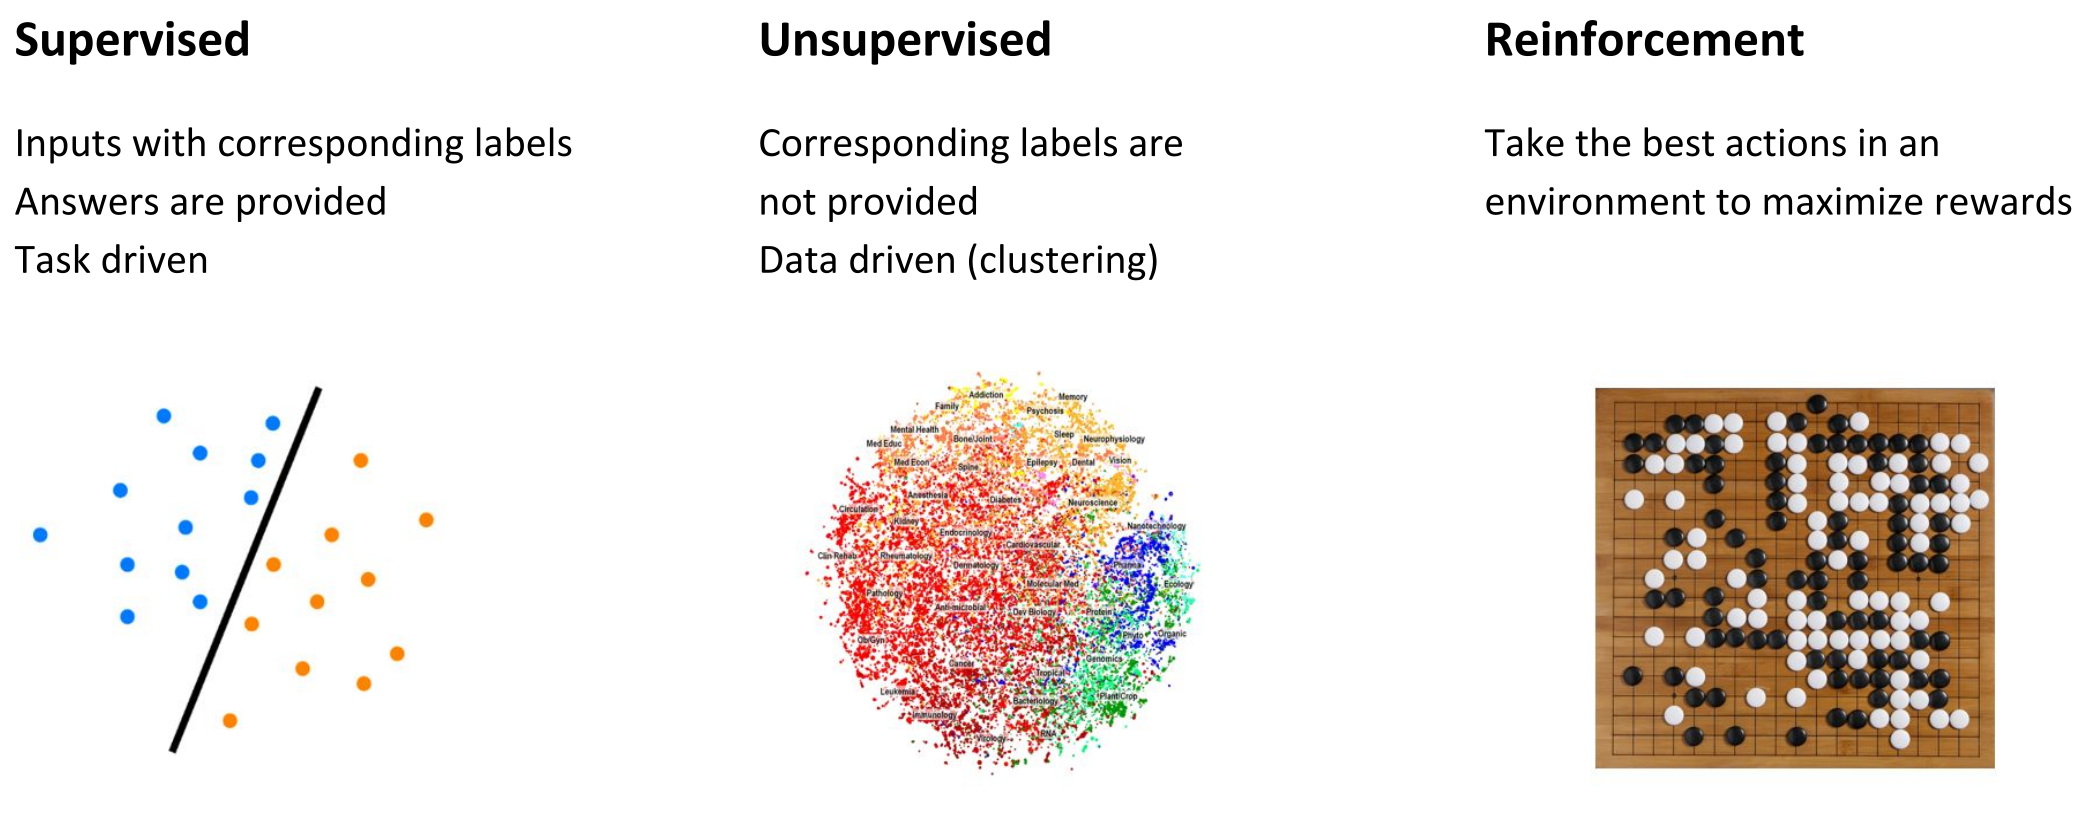
\includegraphics[width=0.5\textwidth]{leeralgoritmes.png}
    \caption{Supervised / Unsupervised / Reinforcement learning}
\end{figure}


\subsection{Supervised Learning}

Leren uit een gelabelde dataset. Vind het verband tussen de features en de labels

\begin{figure}[H]
    \centering
    \includegraphics[width=0.5\textwidth]{supervised-learning.png}
    \includegraphics[width=0.4\textwidth]{supervised-learning2.png}
    \caption{Leren uit een dataset}
\end{figure}

\begin{figure}[H]
    \centering
    \includegraphics[width=0.5\textwidth]{supervised-learning3.png}
    \caption{Supervised learning kan uit ongeziene data een resultaat berekenen}
\end{figure}

\subsubsection{Regressie vs Classificatie}

\begin{figure}[H]
    \centering
    \includegraphics[width=0.5\textwidth]{regressie-vs-classificatie.png}
    \caption{Regressie vs classificatie}
\end{figure}

\begin{figure}[H]
    \centering
    \includegraphics[width=0.5\textwidth]{regressie-vs-classificatie2.png}
    \caption{Regressie vs classificatie}
\end{figure}

\subsubsection{Voorbeeld}

Hoe stuurhoek bepalen bij een self-driving car?

\begin{itemize}
    \item (infrarood) camera's
    \item Stereo vision
    \item Radar
    \item LIDAR
    \item GPS
    \item Audio
\end{itemize}

\begin{figure}[H]
    \centering
    \includegraphics[width=0.6\textwidth]{stuurhoek-selfdriving-car.png}
    \includegraphics[width=0.3\textwidth]{stuurhoek-selfdriving-car2.png}
    \caption{Via sensoren weet de auto }
\end{figure}



\subsection{Unsupervised learning}

\begin{figure}[H]
    \centering
    \includegraphics[width=0.7\textwidth]{unsupervised-learning.png}
    \caption{Unsupervised Learning}
\end{figure}

\begin{figure}[H]
    \centering
    \includegraphics[width=0.5\textwidth]{unsupervised-learning2.png}
    \caption{Voorbeeld Clustering: de data in groepen verdelen}
\end{figure}

\subsection{Reinforcement learning}

\begin{figure}[H]
    \centering
    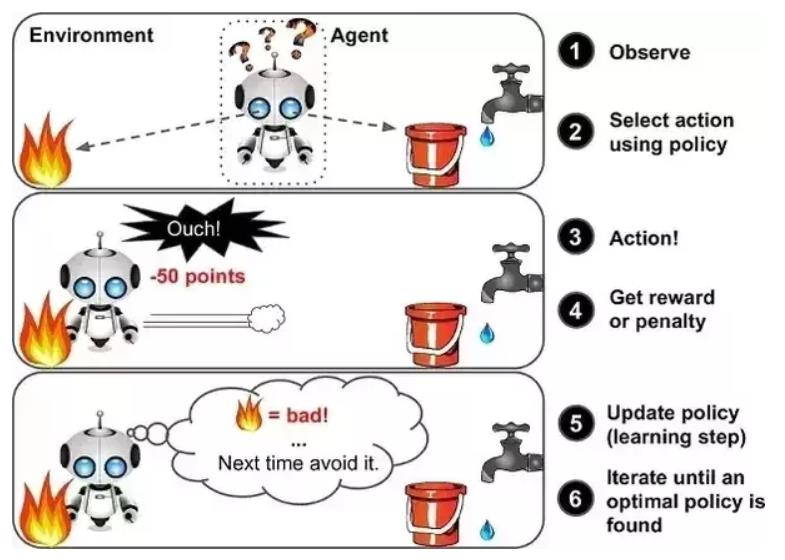
\includegraphics[width=0.5\textwidth]{reinforcement-learning.png}
    \caption{Reinforcement learning}
\end{figure}

\begin{itemize}
    \item Voor elke actie krijgt de AI feedback
    \item De AI leert uit de feedback
    \item In het begin zijn de acties heel willekeurig
\end{itemize}

\subsection{Overzicht leeralgoritmes}

\begin{figure}[H]
    \centering
    \includegraphics[width=0.55\textwidth]{overzicht-leeralgoritmes.png}
    \includegraphics[width=0.5\textwidth]{overzicht-leeralgoritmes2.png}
    \caption{Overzicht}
\end{figure}

\subsection{Werkwijze van een ML Project}

\begin{figure}[H]
    \centering
    \includegraphics[width=0.4\textwidth]{machine-learning-project.png}
    \includegraphics[width=0.35\textwidth]{machine-learning-project2.png}
\end{figure}

\begin{figure}[H]
    \centering
    \includegraphics[width=0.45\textwidth]{machine-learning-project3.png}
\end{figure}

\subsubsection{Tijdverdeling}


\begin{figure}[H]
    \centering
    \includegraphics[width=0.35\textwidth]{machine-learning-project4.png}
    \caption{Tijdverdeling: verwachting vs realiteit}
\end{figure}

\section{Enkelvoudige Lineaire regressie}

\subsection{Voorbeeld}

\begin{figure}[H]
    \centering
    \includegraphics[width=0.3\textwidth]{lineaire-regressie-voorbeeld.png}
    \caption{Voorspel de bloeddruk op basis van leeftijd en gewicht}
\end{figure}

\begin{itemize}
    \item \textbf{features:} leeftijd en gewicht
    \item \textbf{target:} bloeddruk (=wat je wil voorspellen = output = label)
    \item \textbf{trainingset:} 11 training examples (=samples)
\end{itemize}

\begin{theorem}[Regressie-analyse]
Regressie-analyse is het modelleren van of het zoeken naar een verband op basis van één of meerdere variabelen.

Bij regressie is de output/target een (continue) variabele
\end{theorem}

\subsubsection{Scatterplot}

\begin{figure}[H]
    \centering
    \includegraphics[width=0.5\textwidth]{lineaire-regressie-voorbeeld-scatterplot.png}
    \caption{Scatterplot: de grafiek toont een positieve correlatie $\Rightarrow$ een sterk verband}
\end{figure}

\subsection{De hypothese}

\begin{theorem}[De hypothese]
Het verband (model of hypothese) $h_{\theta}(x)$ is van de vorm:

\begin{equation}
h_{\theta}(x) = \theta_0 + \theta_1x
\end{equation}
\end{theorem}

Bepalen van de optimale waarden voor $\theta_0$ en $\theta_1$:

\begin{itemize}
    \item $\theta_0$ = snijpunt van de y-as (= noemen we ook de \textbf{bias})
    \item $\theta_1$ = helling van de rechte (rico)
\end{itemize}

De parameters $\theta_i$ = \textbf{weights}

Het zoeken van het model / hypothese = \textbf{training / learning}

\begin{figure}[H]
    \centering
    \includegraphics[width=0.5\textwidth]{lineaire-regressie-hypothese.png}
    \caption{Lineaire trnedlijn met model $h_{\theta}(x)$}
\end{figure}

$\mathbf{R^2}$\textbf{-waarde:} determinatiecoëfficiënt

\subsection{De kostenfunctie}

We minimaliseren de kostenfunctie $J(\theta)$ via de \textbf{Least Mean Squared} methode (LMS). 

\begin{equation}
J(\theta) = \frac{1}{2\cdot m} \cdot \sum_{i=1}^m (h_{\theta}(x_i) - y_i)^2
\end{equation}

\begin{itemize}
    \item $m =$ de bias $=$ snijpunt met de y-as
    \item De kostenfunctie berekent de gemiddelde fout door alle fouten op te tellen
    \item Elke fout wordt gekwadrateerd om:
    \begin{itemize}
        \item negatieve waardes positief te maken
        \item de fout uit te groten
    \end{itemize}
\end{itemize}

\subsection{Gradient Descent (GDS)}

\begin{equation}
J(\theta_0, \theta_1) = \frac{1}{2\cdot m} \cdot \sum_{i=1}^m ((\theta_1\cdot x_i + \theta_0) - y_i)^2
\end{equation}

Stel de parameters $\theta_0$ en $\theta_1$ voortdurend bij in een iteratief proces 
tot je de waarden voor $\theta_0$ en $\theta_1$ hebt gevonden die de kleinst mogelijke waarde. Start met willekeurige waarden.

\begin{figure}[H]
    \centering
    \includegraphics[width=0.7\textwidth]{gradient-descent-theta0.png}
    \caption{De GDS als $\theta_0 = 0$}
\end{figure}

\begin{itemize}
    \item Je krijgt een dalparabool als uitkomst 
    \item Je kan aflezen wat de parameters moeten zijn om de kleinst mogelijke waarde te vinden
    \item In de realiteit heb je vaak veel meer dan 2 gewichten
    \begin{itemize}
        \item Voorbeeld: de textgenererende AI GPT-3 heeft rond de 175 miljard gewichten 
        \item $\Rightarrow$ veel rekenkracht nodig om beste uitkomst te vinden
    \end{itemize}
\end{itemize}

\subsubsection{Learning rate}

\begin{figure}[H]
    \centering
    \includegraphics[width=0.65\textwidth]{gradient-descent-afgeleiden.png}
    \caption{De parameters $\theta_0$ en $\theta_1$ stellen we constant bij (formules niet te kennen)}
\end{figure}

\begin{itemize}
    \item We bepalen de afgeleide (= de gradient, de helling) van $\theta_0$ en $\theta_1$
    \item We gebruiken die afgeleiden om een betere $\theta_0$ en $\theta_1$ te vinden.
    \item We vermenigvuldigen de gradient met een variable $\eta$ (=de learning rate)
    \item Onze nieuwe $\theta$ wordt berekend met behulp van de oude $\theta$ en de afgeleide maal de learning rate. 
\end{itemize}

\begin{figure}[H]
    \centering
    \includegraphics[width=0.5\textwidth]{lineaire-regressie-learning-rate.png}
    \caption{Learning rate $\eta$: bij een te kleine/te grote $\eta$ hebben we te veel stappen}
\end{figure}

De learning rate $\eta$ stellen we constant bij om met zo weinig aantal stappen het optimum te bereiken.


\section{Meervoudige lineaire regressie}

\begin{theorem}[Meervoudige lineaire regressie]
Bij meervoudige lineaire regressie (multiple regression) wordt het model/hypothese bepaald 
aan de hand van een trainingset met \textbf{meerdere features}.
\end{theorem}

\textbf{Voorbeelden:}

\begin{itemize}
    \item Bloeddruk wordt bepaald a.d.h.v. gewicht en leeftijd
    \item De kwaliteit van wijn wordt voorspeld op basis van: zuurtegraad, suikergehalte, chloriden, dichtheid, sulfaten, hoeveelheid alcohol, \dots
    \item Het warmeverlies van een huis wordt voorspeld op basis van: het type glas, muurisolatie, oriëntatie van het huis, \dots
\end{itemize}

\begin{equation}
h_{\theta}(x) = \theta_0 + \theta_1x_1 + \theta_2x_2 + \dots + \theta_nx_n + 
\end{equation}

\begin{figure}[H]
    \centering
    \includegraphics[width=0.7\textwidth]{multiple-regression-voorbeeld.png}
    \caption{\textbf{Voorbeeld:} voorspel de huisprijs op basis van deze features }
\end{figure}

\subsection{Statistische vooranalyse}

\subsubsection{Consistentie van de dataset}

\begin{itemize}
    \item Volledigheid van de dataset
    \item Inconsistenties
    \item Spreiding van de gegevens
\end{itemize}

Verwijderen van een onnodige kolom:

\begin{minted}{python}
dataset.drop('CHAS', axis=1, inplace=True)
\end{minted}

\subsubsection{Uitschieters}

\begin{itemize}
    \item Vinden en verwijderen van extreme waarden/samples
    \item Geavanceerde technieken: zie later bij clustering
\end{itemize}

\begin{figure}[H]
    \centering
    \includegraphics[width=0.5\textwidth]{multiple-regression-uitschieters.png}
    \caption{Uitschieters}
\end{figure}


\subsubsection{Onderlinge correlatie}

\begin{figure}[H]
    \centering
    \includegraphics[width=0.45\textwidth]{multiple-regression-heatmap.png}
    \includegraphics[width=0.45\textwidth]{multiple-regression-pairplot.png}
    \caption{Heatmap en pairplot van de onderline correlatie tussen de features}
\end{figure}

\subsection{Features en targets}

\begin{figure}[H]
    \centering
    \includegraphics[width=0.5\textwidth]{multiple-regression-features-targets.png}
    \caption{Dataset opsplitsen in features en targets}
\end{figure}

\begin{minted}{python}
# opsplisten in features en targets. axis=1 == column
y = dataset['target_kolom'].values
X = dataset.drop('target_kolom',axis=1).values
# Alternatief: als bvb de laatste kolom het target is
features=list(dataset.columns[:dataset.columns.size-1])
X = dataset[features].values
y = dataset['Price'].values
\end{minted}

\subsection{Trainen van het model}

\begin{figure}[H]
    \centering
    \includegraphics[width=0.35\textwidth]{multiple-regression-training-testset.png}
    \caption{Dataset opsplitsen in training set en test set}
\end{figure}

\begin{itemize}
    \item Belangrijk om eerst de data te randomiseren: te data zou gesorteerd kunnen zijn, dat willen we vermijden
    \item Stel dat huizenprijzen van laag naar hoog gesorteerd is, en je traint de data op de eerste 75\%, en test de laatste 25\%.
    Resultaat: Het model zal niet getraind zijn op dure huizen.
    \item Ander voorbeeld: stel dat je een self-driving AI alleen traint op de autosnelweg, en dan test in een zone-30 straat bij een school...
\end{itemize}


\begin{minted}{python}
X_train, X_test, y_train, y_test = train_test_split(X, y, test_size=0.33, 
random_state=0)
\end{minted}

\subsubsection{Initialiseren en trainen van het regressiemodel}

\begin{minted}{python}
lregmodel = linear_model.LinearRegression()
lregmodel.fit(X_train, y_train)
\end{minted}

Model:

\begin{minted}{python}
print('coeffs: ', lregmodel.coef_)
print('intercept', lregmodel.intercept_)

>> coeffs: [ -3.56141289e+00, 4.05479295 e-01, 8.14080284 e-01, 
    8.96450415 e+01, -3.02997261e-01, -2.77339444e+01, 
    7.47151897 e+00, -2.92233040e-01, -1.61741146e+01, 
    -1.17962045e +01]

>> intercept: 650.652022517
\end{minted}

Price = - 3.56 × CRIM + 0.41 × ZN + 0.81 × INDUS - 270.51 × NOX + 89.65 × RM
- 0.30 × AGE - 27.74 × DIS + 7.47 × RAD - 0.29 × TAX - 16, 17 × PT
+ 0.08 × B - 11.80 × LSTAT + 650.65


\subsection{Testen van het model}

\subsubsection{Voorspellingen maken}

\begin{figure}[H]
    \centering
    \includegraphics[width=0.5\textwidth]{multiple-regression-voorspelling.png}
    \caption{Voorspel de prijs van een huis met deze features}
\end{figure}

\begin{minted}{python}
house = np.array([0.11, 0, 12.03, 0.57, 6.80, 89.30, 2.39, 1, 
273, 21.00, 393.45, 6.48])

house = house.reshape(1, -1)

# met reshape wordt house:
# house = np.array([[0.11, 0, 12.03, 0.57, 6.80, 89.30, 2.39, 1, 
# 273, 21.00, 393.45, 6.48]])

price = lregmodel.predict(house)

print('De prijs van het huis bedraagt: ', price)

>> De prijs van het huis bedraagt: 563.68335073
\end{minted}

\begin{itemize}
    \item reshape(1, -1) maakt een rijvector
    \item Werkelijke prijs: 562.00
\end{itemize}

\subsection{Performantie en scores van het model}

\subsubsection{Mean Absolute Error (MAE)}

\begin{theorem}[MAE]
De Mean Absolute Error (MAE) is \textbf{het gemiddelde van de absolute waarden} van het verschil
tussen de \textbf{werkelijke waarden} $y_i$ en de \textbf{voorspelde waarden} $\hat{y}_i$.

\begin{equation}
\text{MAE} = \frac{1}{n} \cdot \sum_{i=1}^n | y_i - \hat{y}_i |
\end{equation}
\end{theorem}

\begin{minted}{python}
from sklearn.metrics import mean_absolute_error

y_predicted = lgregmodel.predict(X_test)
MAE = mean_absolute_error(y_test, y_predicted)

print('MAE= ', MAE)

>> MAE = 64.0090867586

\end{minted}

\subsubsection{Mean Squared Error (MSE)}

\begin{theorem}[MSE]
De Mean Squared Error (MSE) is \textbf{het gemiddelde van de gekwadrateerde waarden} van het verschil tussen de werkelijke waarden $y_i$ en
de voorspelde waarden $\hat{y}_i$.

\begin{equation}
\text{MSE} = \frac{1}{n} \cdot \sum_{i=1}^n ( y_i - \hat{y}_i )^2
\end{equation}
\end{theorem}

\begin{minted}{python}
from sklearn.metrics import mean_squared_error

y_predicted = lregmodel.predict(X_test)
MSE = mean_squared_error(y_test, y_predicted)

print('MSE = ' MSE)

>> MSE = 7803.89332739
\end{minted}


\subsubsection{Determinatiecoëfficiënt}

\begin{theorem}[De determinatiecoëfficiënt $R^2$]
De determinatiecoëfficiënt ($R^2$) is de variabiliteit van het model

\begin{equation}
R^2 = 1 - \frac{\sum_{i=1}^n (y_i - \hat{y}_i)^2 }{\sum_{i=1}^n (y_i - \bar{y})^2}
\end{equation}

Bij perfecte voorspellingen is $R^2 = 1$

Een negatieve waarde voor $R^2$ betekent dat het model slechter scoort dan een horizontale lijn (= slechter dan het gemiddelde te nemen) ($y_i = \bar{y}$, $\bar{y}$ is het gemiddelde van y)
\end{theorem}

\begin{minted}{python}
from sklearn.metrics import r2_score

y_predicted = lregmodel.predict(X_test)
r2 = r2_score(y_test, y_predicted)

print('r2_score = ', r2)

# alternatieve manier voor het bepalen van de r2 score:
r2 = lregmodel.score(X_test, y_test)

>> r2 score = 0.754254234917
\end{minted}

\section{Feature engineering}

Om een beter model te verkrijgen (en zo een betere $R^2$ score), kunnen we verschillende dingen doen:

\begin{itemize}
    \item Meer data toevoegen
    \item Ander model kiezen, hyperparameter tuning
    \item Feature engineering: het aanmaken van extra features gebaseerd op de bestaande features
\end{itemize}

\subsection{Normalisatie / Scaling}

\begin{theorem}[Normalisatie / Scaling]
Normalisatie of Scaling zorgt ervoor dat de features op dezelfde schaalverdeling staan
\end{theorem}

In ons voorbeeld van de huurprijs:

\begin{figure}[H]
    \centering
    \includegraphics[width=0.6\textwidth]{normalisatie.png}
    \caption{NOX: min = 0.385, max = 0.871; TAX: min = 188, max = 711}
\end{figure}

\subsubsection{Voordelen}

\begin{figure}[H]
    \centering
    \includegraphics[width=0.4\textwidth]{scaling.png}
    \caption{Gradient Descent convergeert minder snel als features op een verschillende schaalgrootte staan. Normalisatie zorgt er dus voor dat het model sneller zal trainen.}
\end{figure}

\subsubsection{MIN-MAX-scaling}

\begin{equation}
x_{s_i} = \frac{x_i - Min(x)}{Max(x) - Min(x)}
\end{equation}

\begin{itemize}
    \item Schaalt alle features tussen 0 en 1
    \item Werkt goed bij niet-Gaussiaanse distributies en bij kleine variantie
    \item De scheefheid (skew) blijft bewaard
    \item Gevoelig voor uitschieters
\end{itemize}

\begin{figure}[H]
    \centering
    \includegraphics[width=0.4\textwidth]{min-max-scaling.png}
    \caption{Voor en na scaling}
\end{figure}

\begin{figure}[H]
    \centering
    \includegraphics[width=0.4\textwidth]{min-max-houses.png}
    \caption{Bij het voorbeeld van de huizenprijzen}
\end{figure}

\begin{minted}{python}
from sklean.preprocessing import MinMaxScaler

scaler = MinMaxScaler().fit(X_train)
X_train = scaler.transform(X_train)
X_test = scaler.transform(X_test)

# alternatief
scaler = MinMaxScaler()
X_train = scaler.fit_transform(X_train)
X_test = scaler.transform(X_test)
\end{minted}

\subsubsection{Standard scaling (normalisatie)}

\begin{equation}
x_{s_i} = \frac{x_i - mean(x)}{stdev(x)}
\end{equation}

\begin{itemize}
    \item Geschaalde features;
    \begin{itemize}
        \item Gemiddelde = 0
        \item Standaardafwijking = 1
    \end{itemize}
    \item Geschaalde features schommelen rond 0 (soms nodig bij deep learning)
    \item Vervormt geen relatieve afstanden tussen de feature waarden
    \item Kan beter overweg met uitschieters
    \item Garandeert geen genormaliseerde data op exact dezelfde schaal
\end{itemize}

\begin{figure}[H]
    \centering
    \includegraphics[width=0.4\textwidth]{standard-scaling.png}
    \caption{Voor en na standard scaling}
\end{figure}

\begin{figure}[H]
    \centering
    \includegraphics[width=0.4\textwidth]{standard-scaling-houses.png}
    \caption{Bij het voorbeeld van de huizenprijzen}
\end{figure}


\begin{minted}{python}
from sklean.preprocessing import StandardScaler

scaler = StandardScaler().fit(X_train)
X_train = scaler.transform(X_train)
X_test = scaler.transform(X_test)

# alternatief
scaler = StandardScaler()
X_train = scaler.fit_transform(X_train)
X_test = scaler.transform(X_test)
\end{minted}

\subsubsection{Robust scaling}

\begin{equation}
x_{s_i} = \frac{x_i - Q_2(x)}{Q_3(x) - Q_1(x)}
\end{equation}

\begin{itemize}
    \item Lijkt op MIN-MAX scaler maar gebruikt de interkwartielafstand ipv range
    \item Houdt geen rekening met uitschieters
    \item Gebruikt minder data bij het bepalen van de schaal
    \item Range van de genormaliseerde data is groter dan bij MIN-MAX scaling
    \item Garandeert geen genormaliseerde data op exact dezelfde schaal
\end{itemize}

\begin{figure}[H]
    \centering
    \includegraphics[width=0.45\textwidth]{robust-scaling.png}
    \includegraphics[width=0.45\textwidth]{robust-scaling2.png}
    \caption{Voor en na robust scaling}
\end{figure}

\begin{minted}{python}
from sklean.preprocessing import RobustScaler

scaler = RobustScaler().fit(X_train)
X_train = scaler.transform(X_train)
X_test = scaler.transform(X_test)

# alternatief
scaler = RobustScaler()
X_train = scaler.fit_transform(X_train)
X_test = scaler.transform(X_test)
\end{minted}

\subsection{Feature expansion}

\subsubsection{Nieuwe features}

Bedenken van nieuwe features

\textbf{Voorbeelden:}

\begin{itemize}
    \item Uit de lengte en breedte van een huis de oppervlakte halen als nieuwe feature.
    \item Uit een start en eindpunt de afstand halen als nieuwe feature.
    \item Uit een datum afleiden welke dag van de week het is.
    \item Veranderingen in de features.
    \item Nieuwe opgemeten parameters.
\end{itemize}

\subsubsection{Hogere-orde features}

= Het verband tussen features en de target(s) is niet altijd lineair.

\textbf{Voorbeeld:} samenhang tussen LSTAT $(x_1)$ en de huizenprijs $(P)$

\begin{figure}[H]
    \centering
    \includegraphics[width=0.3\textwidth]{hogere-orde-features.png}
    \caption{$P = \theta_0 + \theta_1x_1$}
\end{figure}

Toevoegen van een extra hogere-orde feature $x_2 = x^2_1$:

\begin{figure}[H]
    \centering
    \includegraphics[width=0.3\textwidth]{hogere-orde-features2.png}
    \caption{$P = \theta_0 + \theta_1x_1 + \theta_2x_2$ }
\end{figure}

Toevoegen van een extra hogere-orde features $x_3 = x^3_1$ en $x_4 = x^4_1$:

\begin{figure}[H]
    \centering
    \includegraphics[width=0.3\textwidth]{hogere-orde-features3.png}
    \caption{$P = \theta_0 + \theta_1x_1 + \theta_2x_2 + \theta_3x_3$ }
    \includegraphics[width=0.3\textwidth]{hogere-orde-features4.png}
    \caption{$P = \theta_0 + \theta_1x_1 + \theta_2x_2 + \theta_3x_3 + \theta_4x_4$}
\end{figure}

\begin{figure}[H]
    \centering
\end{figure}

\begin{minted}{python}
# toevoegen van een extra feature: LSTAT^2 LSTAT^3
dataset.insert(dataset.columns.size - 1, 'LSTAT^2', dataset.LSTAT**2)
dataset.insert(dataset.columns.size - 1, 'LSTAT^3', dataset.LSTAT**3)
\end{minted}

\begin{figure}[H]
    \centering
    \includegraphics[width=0.7\textwidth]{hogere-orde-features5.png}
    \caption{Resultaat toevoegen hogere-orde features}
\end{figure}

\begin{itemize}
    \item Nu model met extra features trainen en nadien testen op de test set.
    \item \textbf{Opgepast:} bij de test set moet je ook dezelfde features toevoegen.
\end{itemize}

\subsection{One-hot encoding}

\begin{itemize}
    \item = Omzetten van categorische variabelen naar meerdere aparte features
    \item categorische variabelen = variabelen zonder echte waarden, de waarden stellen een categorie voor (niet altijd een nummer)
    \item $\Rightarrow$ voor elke categorie een nieuwe kolom
    \item `Dummy Variable Trap'
    \begin{itemize}
        \item = als een rij maar tot 1 categorie kan behoren (zie onderstaand voorbeeld, een appel is geen kip), dan zou je in principe 1 kolom kunnen schrappen en dan kan je toch dezelfde informatie krijgen.
        \item $x_1 + x_2 + x_3 = 1 \Leftrightarrow x_1 = 1 - x_2 - x_3$   
        \item In de praktijk laat men dit gewoon staan.
        \item (niet te kennen op examen)
    \end{itemize}
\end{itemize}

\begin{figure}[H]
    \centering
    \includegraphics[width=0.6\textwidth]{one-hot-encoding.png}
    \caption{Voorbeeld One-hot encoding}
\end{figure}

\begin{minted}{python}
# voeg de categorieen toe als kolommen
dataset = pd.concat(
    [dataset, pd.get_dummies(dataset['food_name'], prefix='food')], 
    axis=1)
# verwijder de food_name kolom
dataset.drop(['food_name'], axis=1, inplace=True)
# toon de eerste 5 rijen:
dataset.head()
\end{minted}

\begin{figure}[H]
    \centering
    \includegraphics[width=0.7\textwidth]{one-hot-encoding2.png}
    \caption{Resultaat van dataset.head(), voor en na one-hot encoding}
\end{figure}

\section{Underfitting \& overfitting}

\subsection{Underfitting}

\begin{theorem}[Underfitting]
Underfitting treedt op wanneer een model de training data niet kan modelleren 
en ook niet kan generaliseren op nieuwe data.

\begin{itemize}
    \item Het model is te 'simpel'
    \item Model met hoge bias
    \item $\Rightarrow$ de score met de training data en de score met de test data zijn beiden laag.
\end{itemize}
\end{theorem}

\begin{figure}[H]
    \centering
    \includegraphics[width=0.5\textwidth]{underfitting.png}
    \caption{Het model werkt voor sommige variabelen maar voor velen ook niet}
\end{figure}

\subsection{Overfitting}

\begin{theorem}[Overfitting]
Overfitting treedt op wanneer een model de training data te goed modelleert en niet kan
    generaliseren op nieuwe data.  

\begin{itemize}
    \item Het model is te 'complex'
    \item De ruis van willekeurige fluctuaties in data worden opgepikt
    \item Model met een hoge variance
    \item $\Rightarrow$ de score met de training data is groter dan de score met de test data
\end{itemize}
\end{theorem}

\begin{figure}[H]
    \centering
    \includegraphics[width=0.5\textwidth]{overfitting.png}
    \caption{Model met order $\approx 15$}
\end{figure}

\subsubsection{Impact van de grootte van de dataset}

Afhankelijkheid van de grootte van de dataset (aantal observaties $m$):

\begin{itemize}
    \item Bij weinig observaties: snel overfitting bij complexer model
    \item Bij veel observaties: minder snel overfitting bij complexer model
\end{itemize}

\begin{figure}[H]
    \centering
    \includegraphics[width=0.5\textwidth]{overfitting2.png}
    \caption{Voorbeeld met 3de orde polynoom: links = overfitting, rechts niet}
\end{figure}

\subsection{Regularisatie (regularisation)}

\begin{theorem}[Regularisatie]
Methode om de mate van bias van een hypothese te regelen en een 
goed evenwicht te vinden tussen underfitting en overfitting.

We gebruikten tot nu een kostenfunctie die we moesten minimaliseren om het model te trainen. Daar voegen we nu $R(\theta)$ aan toe:

\begin{equation}
J(\theta) = \frac{1}{2\cdot m} \sum_{i=1}^m (h_{\theta}(x_i) - y_i)^2 + R(\theta)
\end{equation}
\end{theorem}

\begin{theorem}[$R(\theta)$]
$R(\theta)$ is de regularisatie-term. 

Dit is een extra kostenterm die het gebruik van hogere orde features afstraft
tenzij ze de globale kostenfunctie doen dalen. $R(\theta)$ is gelijk aan $\lambda \theta \theta^{\tau}$.
\end{theorem}

\subsubsection{Voorbeeld regularisatie}

\begin{center}
    $J(\theta) = \frac{1}{2\cdot m} \sum_{i=1}^m (h_{\theta}(x_i) - y_i)^2 + \lambda \theta \theta^{\tau}$
\end{center}

\begin{itemize}
    \item $\theta = \{\theta_1, \dots, \theta_n\}$
    \begin{itemize}
        \item intercept $\theta_0$ wordt meestal niet geregulariseerd
        \item Als de $\theta$'s vergroten, zal de $R(\theta)$ ook vergroten
    \end{itemize}
    \item $\lambda$ is een tuning parameter (hyper parameter), we moeten die zelf vinden
    \begin{itemize}
        \item $\lambda = 0 \Rightarrow$ geen regularisatie
        \item $\lambda = \inf \Rightarrow \theta = 0$ 
        \item $\lambda$ tussenin regelt de mate van regularisatie.
    \end{itemize}
\end{itemize}

De tuningparameter $\lambda$ regelt de complexiteit van de hypothese:

\begin{itemize}
    \item Kleine waarde voor $\lambda$: lage bias, hoge variantie (overfitting)
    \item Grote waarde voor $\lambda$: hoge bias, lage variantie (underfitting)
\end{itemize}

Afhankelijk van hoe $R$ gedefinieerd wordt is er een andere benaming voor de regularisatie:

\begin{itemize}
    \item Ridge regression (L2 regularisatie)
    \item Lasso regression (L1 regularisatie)
\end{itemize}

Het is ook mogelijk om meerdere regularisatietermen aan de kostenfunctie toe te voegen, 
bijvoorbeeld 1 gebaseerd op L2 en 1 op L1.

\subsubsection{Regularisatie met L2 norm}

Bij L2 regularisatie wordt de regularisatieterm berekend met behulp van de som 
van de kwadraten van de $\theta$'s 

\begin{center}
$J_{L2} = J + \lambda_2 \sum_{j=1}^m \theta_j^2$

$J_{L2} = \sum_{i=1}^n (\text{target}_i - \text{output}_i) + \lambda_2 \sum_{j=1}^m \theta_j^2$
\end{center}


\subsubsection{Regularisatie met L1 norm}

Bij L2 regularisatie wordt de regularisatieterm berekend met behulp van de som 
van de absolute waardes van de $\theta$'s 

\begin{center}
$J_{L1} = J + \lambda_1 \sum_{j=1}^m |\theta_j|$

$J_{L1} = \sum_{i=1}^n (\text{target}_i - \text{output}_i) + \lambda_1 \sum_{j=1}^m |\theta_j|$
\end{center}


\subsubsection{Voorbeeld regularisatie op huizenprijzen}

Via Ridge of Lasso regressie met regularisatieparameter $\alpha$

\begin{itemize}
    \item Hoe groter $\alpha$, hoe sterker de regularisatie en dus hoe simpler het model
    \item Hoe kleiner $\alpha$, hoe zwakker de regularisatie en dus hoe complexer het model
\end{itemize}

\begin{minted}{python}
regmodel = Ridge(alpha=0.14, tol=0.0001, fit_intercept=True)
regmodel.fit(X_train, y_train)
regmodel.score(X_test, y_test)
>> 0.79834480089914472

lregmodel = Lasso(alpha=0.5, tol=0.0001, fit_intercept=True)
lregomdel.fit(X_train, y_train)
lregmodel.score(X_test, y_test)
>> 0.8437113338085345
\end{minted}

\section{Classificatie}

\subsection{Wat is classificatie?}

\begin{theorem}[Classificatie]
Classificatie is een supervised learning techniek waarbij een getraind model
niet-geziene inputs toewijst aan één of meerdere gelabelde categorieën (classes)
\end{theorem}

\subsubsection{Voorbeelden}

\begin{itemize}
    \item Gezichtsherkenning
    \item Nummerplaatherkenning
    \item Spam detectie
    \item Medische diagnoses
    \item Voorspelling of een klant op een advertentie zal klikken
    \item Kwaliteitscontrole
    \item \dots
\end{itemize}

\begin{figure}[H]
    \centering
    \includegraphics[width=0.4\textwidth]{classificatie-gezichtsherkenning.png}
    \caption{Geslachtsherkenning + leeftijdsclassificatie}
\end{figure}


\subsection{Types van classifiers}

\subsubsection{Binary (binomial) classifier}

= verdeel de samples in \textbf{twee verschillende klasses}

\begin{figure}[H]
    \centering
    \includegraphics[width=0.3\textwidth]{binary-class.png}
    \caption{Voorbeeld: bepaal of een kanker goedaardig of kwaadaardig is}
\end{figure}

\subsubsection{Multiclass classifier}

\begin{theorem}
    Een multiclass classifier zal samples in 3 of meer verschillende klasses verdelen
\end{theorem}

\begin{figure}[H]
    \centering
    \includegraphics[width=0.5\textwidth]{multiclass-classifier.png}
    \caption{Voorbeelden: gezichtsherkenning, sentiment analyse}
\end{figure}

\subsubsection{Multilabel classifier}

\begin{theorem}
    Een multilabel classifier zal meerdere labels aan een sample toewijzen.
    Een sample kan dus tot meerdere klasses behoren
\end{theorem}

\begin{figure}[H]
    \centering
    \includegraphics[width=0.5\textwidth]{multilabel-classifier.png}
    \caption{Image content analysis, een film kan tot meerdere genres behoren}
\end{figure}

\subsection{Voorbeeld van een classificatie: appel herkennen}

\begin{figure}[H]
    \centering
    \includegraphics[width=0.2\textwidth]{multilabel-classifier2.png}
    \caption{Voorspel of een stuk fruit een appel is op basis van vorm en kleur}
\end{figure}

\begin{itemize}
    \item features: rondheid en groenheid
    \item target: appel: ja/nee
    \item trainingset: 15 training samples
\end{itemize}

Bij classificatie is de output/target een \textbf{(discrete) variabele/klasse}

\begin{figure}[H]
    \centering
    \includegraphics[width=0.5\textwidth]{multilabel-classifier3.png}
\end{figure}

\subsubsection{Waarom lineaire regressie geen goede optie is}

\begin{figure}[H]
    \centering
    \includegraphics[width=0.5\textwidth]{classificatie-regressie.png}
    \caption{Voorbeeld: rondheid bepaalt of het een appel is of niet}
\end{figure}

\begin{figure}[H]
    \centering
    \includegraphics[width=0.5\textwidth]{classificatie-regressie2.png}
    \caption{We proberen te classificeren met behulp van lineaire regressie}
\end{figure}

\begin{figure}[H]
    \centering
    \includegraphics[width=0.5\textwidth]{classificatie-regressie3.png}
    \caption{Toeveogen van een nieuw punt (rechts)}
\end{figure}

\begin{itemize}
    \item Stel dat we een nieuw punt toevoegen dan kan het zijn dat onze regressie veel minder nauwkeurig is
    \item Een betere manier: \textbf{logistische regressie}
\end{itemize}

\section{Logistische regressie}

\begin{theorem}
    Logistische regressie wordt gebruikt om de kans te bepalen of een bepaalde sample 
    tot één van twee klasses behoort. De uitkomst is dus een probabiliteit. 
    
    De naam is een beetje misleidend: Logistic Regression is eigenlijk een classificatietechniek. 
    De reden voor deze naam is omdat regressie gebruikt wordt om de classificatie te berekenen.
\end{theorem}

\subsection{Het model}

Omdat de uitkomst een probabiliteit is, zoeken we een functie $h_{\theta}$ zodat het model $h_{\theta}(x)$ voldoet aan:

\begin{center}
$0 \leq h_{\theta}(x) \leq 1$
\end{center}

\begin{itemize}
    \item $h_{\theta}(x)$ = de geschatte kans dat $y=1$ bij input $x$
    \item Voorbeeld: $h_{\theta}(x) = 0.80$
    \begin{itemize}
        \item Het model is voor 80\% overtuigd dat het om een appel gaat.
        \item Als je dus als threshold 50\% gebruikt, classificeert het model het object als een appel
    \end{itemize}
\end{itemize}

\subsubsection{De logistische functie}

\begin{equation}
h_{\theta}(x) = \frac{1}{1 + e^{-\theta^{\tau}x}}
\end{equation}

\begin{itemize}
    \item Met $e =$ het getal van Euler = $\approx 2.718$
    \item Dit is een sigmoïdefunctie: de basisvorm voor zo'n functie is $\frac{1}{1+e^{-z}}$
    \item Bij onze logistische functie is $z$ dus gelijk aan $\theta^{\tau}x$
    \begin{itemize}
        \item Dit is gelijk aan de uitkomst van een lineaire regressiefunctie
        \item Met $x =$ de samplewaardes
        \item Met $\theta =$ de gewichten die bij die waardes horen 
    \end{itemize}
\end{itemize}

\begin{figure}[H]
    \centering
    \includegraphics[width=0.3\textwidth]{logistic-regression.png}
    \caption{De logistische functie is duidelijk een sigmoïdefunctie of S-functie}
\end{figure}

\begin{itemize}
    \item $y=1$ als $h_{\theta}(x) \geq 0.5 \Rightarrow \theta^{\tau}x \geq 0$
    \item $y=0$ als $h_{\theta}(x) < 0.5 \Rightarrow \theta^{\tau}x < 0$
\end{itemize}

\subsubsection{Interpretatie via voorbeeld appels}

Het model is van de vorm:

\begin{center}
    $h_{\theta}(x) = g(\theta_0 + \theta_1x_1 + \theta_2x_2)$

    met $x_1=$ rondheid en $x_2=$ groenheid
\end{center}

Veronderstel na training: $\theta_0=-40, \theta_1=4, \theta_2=4$

\begin{itemize}
    \item Voorspel $y=1$ als $-40 + 4x_1 + 4x_2 \geq 0$
    \item Voorspel $y=0$ als $-40 + 4x_1 + 4x_2 < 0$
\end{itemize}

Gegeven een rondheid van 8 en een groenheid van 6:

\begin{center}
    $-40 + 4 \cdot 8 + 4 \cdot 6 = 16 \Rightarrow $ Appel

    $h_{\theta}(x) = \frac{1}{1 + e^{-16}} = 0.999999887$
\end{center}

Gegeven een rondheid van 5 en een groenheid van 4.5:

\begin{center}
    $-40 + 4 \cdot 5 + 4 \cdot 4.5 = -2 \Rightarrow $ Geen appel

    $h_{\theta}(x) = \frac{1}{1 + e^{-2}} = 0.12$
\end{center}

\begin{itemize}
    \item Het model is maar voor 12\% zeker dat het om een appel gaat
    \item $\Rightarrow$ Met 88\% zekerheid gaat het volgens het model niet om een appel
\end{itemize}

\subsubsection{Grafische interpretatie via voorbeeld appels}

\begin{itemize}
    \item Op de scheidingslijn: $\theta_0 + \theta_1x_1 + \theta_2x_2 = 0$
    \item In het voorbeeld: $-40 + 4x_1 + 4_x2 = 0$
\end{itemize}

\begin{figure}[H]
    \centering
    \includegraphics[width=0.4\textwidth]{logistic-grafische.png}
    \caption{}
\end{figure}

\subsubsection{Wat als het model niet lineair is?}

\begin{figure}[H]
    \centering
    \includegraphics[width=0.3\textwidth]{logistic-circle.png}
    \caption{Het model is niet lineair}
\end{figure}


Extra features: $h_{\theta}(x) = g(\theta_0 + \theta_1x_1 + \theta_2x_2 + \theta_3x_1^2 + \theta_4x_4^2)$

\begin{itemize}
    \item Veronderstel: $\theta_0 = -2, \theta_1 = 0, \theta_2 = 0, \theta_3 = 1, \theta_4 = 1$
    \item Voorspel $y=1$ als $-2 + x_1^2 + x_2^2 \geq 0$
\end{itemize}

\begin{figure}[H]
    \centering
    \includegraphics[width=0.3\textwidth]{logistic-circle2.png}
    \caption{$x_1^2 + x_2^2 \geq 2$ (vergelijking van een cirkel met straal $\sqrt{2}$)}
\end{figure}

\subsection{De kostenfunctie}

De kostenfunctie wordt:

\begin{equation}
J(\theta) = \left\{
    \begin{array}{ll}
        -ln(h_\theta(x))\ \text{als}\ y = 1\\
        -ln(1 - h_\theta(x))\ \text{als}\ y = 0\\
    \end{array}
\right.
\end{equation}

\begin{equation}
J(\theta) = -\frac{1}{m} \cdot \Bigg[ \sum_{i=1}^m y_i ln(h_{\theta}(x_i)) + (1 - y_i) \cdot ln(1 - h_{\theta}(x_i)) \Bigg]
\end{equation}

\begin{figure}[H]
    \centering
    \includegraphics[width=0.5\textwidth]{logistic-kostenfunctie.png}
    \caption{Zoek de waarden voor $\theta$ die de kostenfunctie $J(\theta)$ minimaliseert via Gradient Descent (GDS)}
\end{figure}

\subsection{Voorbeeld logistic regression met Sklearn (lineair model)}

\subsubsection{Preprocessing van de data}

Analoog aan preprocessing bij lineaire regressie:

\begin{itemize}
    \item Data inlezen
    \item Check op inconsistenties
    \item Check uitschieters
    \item Plot de data
    \item Splits op in features en targets
    \item Verdeel in een training en test set
\end{itemize}

\begin{minted}{python}
# importeer de dataset
dataset = pd.read_csv('appels.csv')
# definieer de features
features = list(dataset.columns[:dataset.columns.size-1])
X = dataset[features].values
y = dataset['appel'].values
# lettergrootte voor de axis labels
sns.set(font_scale=2) 
# definieer kleuren
colors = ['blue', 'red', 'greyish', 'faded_green', 'dusty_purple']
# plot
sns.lmplot(x='rondheid', y='groenheid', data=dataset, 
    fit_reg=False,  hue='appel', palette=sns.xkcd_palette(colors), 
    scatter_kws={'s': 500}, size=7, aspect=1.5)
\end{minted}

\begin{figure}[H]
    \centering
    \includegraphics[width=0.5\textwidth]{logistic-sklearn-preprocessing.png}
    \caption{Plot van de dataset}
\end{figure}


\subsubsection{Trainen van het logistic regression model}

\begin{minted}{python}
# train een logistic regression classifier
logreg = linear_model.LogisticRegression(C=1e5)
# C = inverse of regularisation strength
# must be a positive float
# like in support vector machines: smaller values => stronger regularisation
logreg.fit(X, y)

print('coefficienten: ', logref.coef_)
print('intercept: ', logreg.intercept_)

\end{minted}

\begin{itemize}
    \item Coefficienten: $\theta_1 = 4.287$ en $\theta_2 = 4.062$
    \item Intercept: $\theta_0 = -43.941$
\end{itemize}

\subsubsection{Classificeren van een nieuwe sample}

\begin{minted}{python}
# voorspel de klasse met rondheid = 8 en groenheid = 6
print(logreg.predict(np.array([8,6]).reshape(1, -1)))

kans = logreg.predict_proba(np.array([8,6]).reshape(1, -1))
print("Kans op appel/geen appel = ", kans)

# voorspel de klasse met rondheid = 4 en groenheid = 4
print(logreg.predict(np.array([4,4]).reshape(1, -1)))

kans = logreg.predict_proba(np.array([4,4]).reshape(1, -1))
print("Kans op appel/geen appel = ", kans)
\end{minted}

Output:

\begin{itemize}
    \item kans op een appel/geen appel: 3.99395302e-07 | 9.99999601e-01
    \item kans op een appel/geen appel: 9.99973583e-01 | 2.64168196e-05
\end{itemize}

\subsubsection{Visualiseer de decision boundary}

\begin{minted}{python}
h = 0.01
rond_min = X[:,0].min()-2
rond_max = X[:,0].max()+2
groen_min = X[:,1].min()-2
groen_max = X[:,1].max()+2
xx, yy = np.meshgrid(np.arange(rond_min, rond_max, h),np.arange(groen_min, groen_max, h))
Z = logreg.predict(np.c_[xx.ravel(), yy.ravel()])
Z = Z.reshape(xx.shape)
# font settings
sns.set(font_scale = 2)
# colors
colors = ["blue", "red", "greyish", "faded green", "dusty purple"]
sns.lmplot(x='rondheid',y='groenheid',data=dataset,
    fit_reg=False,hue='appel',palette=sns.xkcd_palette(colors),
    scatter_kws={'s':200}, height=8, aspect=1.5)
plt.ylim(0, 11)
plt.xlim(0, 11)
plt.contour(xx, yy, Z, colors='green')
\end{minted}

\begin{figure}[H]
    \centering
    \includegraphics[width=0.5\textwidth]{logistic-sklearn-decision-boundary.png}
    \caption{Visualisatie van de decision boundary}
\end{figure}

\subsection{Voorbeeld logistic regression met Sklearn - niet-lineair}

\begin{figure}[H]
    \centering
    \includegraphics[width=0.4\textwidth]{logistic-non-linear.png}
    \caption{Niet-lineair scheidbare dataset}
\end{figure}

\subsubsection{Feature engineering: automatisch toevoegen van hogere orde features}

\begin{minted}{python}
# Aanmaken van de hogere orde features
graad = 3

poly = PolynomialFeatures(graad)
Xp = poly.fit_transform(X)

# Train model op hogere orde features en visualiseer de decision boundary
logreg_poly = linear_model.LogisticRegression(C=1)
logreg_poly.fit(Xp, y)
\end{minted}

\begin{figure}[H]
    \centering
    \includegraphics[width=0.5\textwidth]{logistic-non-linear2.png}
    \caption{Resultaat: overfitting}
\end{figure}


\subsubsection{Oplossing: regularisatie}

\begin{figure}[H]
    \centering
    \includegraphics[width=0.5\textwidth]{logistic-fitting.png}
    \caption{Regelen tussen underfitting en overfitting via regularisatie}
\end{figure}

\begin{itemize}
    \item Via regularisatie een goed evenwicht zoeken tussen underfitting en overfitting
    \item In Scikit Learn linear\_model.LogisticRegression:
    \begin{itemize}
        \item C = inverse regularisatie sterkte
        \item kleine waarden voor C $\Rightarrow$ sterke regularisatie (overfitting)
        \item grote waarden voor C $\Rightarrow$ zwakke regularisatie (underfitting)
    \end{itemize}
\end{itemize}

\begin{minted}{python}
logreg = linear_model.LogisticRegression(C=100)
logreg.fit(Xf, y)
\end{minted}

\subsection{Multi-class classification}

Data kan tot meerdere klasses behoren.
We kunnen met zo'n data dus geen binaire classificatie doen.


\subsubsection{One-vs-All}

\begin{figure}[H]
    \centering
    \includegraphics[width=0.5\textwidth]{multi-class-classification.png}
    \caption{One-vs-All: we maken 3 binaire classifiers}
\end{figure}


\begin{itemize}
    \item `One-vs-Rest'
    \item Je classificeert 1 klasse tegen de rest
    \item Je hebt dus 1 classifier per klasse
    \item Totaal aantal classifiers: N (met N = aantal klasses)
    \item Gevoeliger voor niet-gebalanceerde data (als er in een bepaalde klasse weinig datasamples zijn)
\end{itemize}

\subsubsection{One-vs-One}

\begin{figure}[H]
    \centering
    \includegraphics[width=0.4\textwidth]{multi-class-classification2.png}
    \caption{One-vs-One}
\end{figure}

\begin{itemize}
    \item Je hebt $\frac{N\cdot(N-1)}{2}$ classifiers (met N = aantal klasses) $\Rightarrow$ rekenintensiever dan One-vs-All
    \item Minder gevoelig voor niet-gebalanceerde data
\end{itemize}

\section{Evaluatie van een classifier}

We moeten kunnen bepalen hoe goed een classifier is, om te weten hoe betrouwbaar de voorspelling is
en om de classifier te vergelijken met andere classifiers. 
Bij regressie kunnen we gebruikmaken van onder andere MAE, MSE en de determinatiecoëfficiënt.
 
Bij classificatie zijn die metrics niet interpreteerbaar. 
Daarom maken we gebruik van andere metrics die allemaal berekend worden met behulp van een waarheidstabel:

\begin{figure}[H]
    \centering
    \includegraphics[width=0.4\textwidth]{truth-table.png}
    \caption{Confusion matrix}
\end{figure}

Stel: we hebben een binaire classifier die klasse 0 of 1 als output heeft.
We vergelijken de verwachte waarden uit de classifier met de werkelijke waardes uit de testset.

\begin{itemize}
    \item True Positive = de verwachte waarde en werkelijke waarde zijn beide 1
    \item False Positive = de verwachte waarde is 1, terwijl de werkelijke waarde 0 is
    \item False Negative = de verwachte waarde is 0, terwijl de werkelijke waarde 1 is
    \item True Negative = de verwachte waarde en werkelijke waarde zijn beide 0
\end{itemize}

We tellen het aantal TP, FP, FN, TN om te gebruiken in de volgende formules. 
Deze formules kunnen we gebruiken om een classifier te evalueren.

\subsection{Accuracy}

\begin{equation}
    \text{Accuracy} = \frac{TP + TN}{TP + FP + FN + TN}
\end{equation}

\textbf{Probleem:} stel dat TN = 990, FN = 10, TP = 0, FP = 0

\begin{itemize}
    \item Dan heb je een accuracy van 99\%, terwijl je eigenlijk geen enkele positieve predictie hebt
    \item Accuracy is dus niet altijd veelzeggend $\Rightarrow$ nood aan andere termen
\end{itemize}

\subsection{True Positive Rate (TPR)}

= Recall = Sensitivity = Hit rate

\begin{equation}
    \text{Recall} = \frac{TP}{TP + FN}
\end{equation}

\begin{itemize}
    \item = Het aantal juiste positieve voorspellingen op het totaal aantal positieve waarden in werkelijkheid
    \item Wordt vaak in combinatie gebruikt met Precision (PPV)
\end{itemize}


\subsection{Positive Predictive Value (PPV)}

= Precision

\begin{equation}
    \text{Precision} = \frac{TP}{TP + FP}
\end{equation}

\begin{itemize}
    \item = Het aantal juiste positieve voorspellingen op het totaal aantal positieve voorspellingen
\end{itemize}

\subsection{F1 Score}

\begin{equation}
    \text{F1 score} = \frac{2\cdot(\text{Recall} \cdot \text{Precision})}{(\text{Recall} + \text{Precision})}
\end{equation}

\begin{itemize}
    \item Is een harmonisch gewogen gemiddelde van de recall en de precision
    \item Is de $F_\beta$-score met $\beta = 1$ : $F_{\beta} = \frac{(1+\beta^2)*\text{Precision}*\text{Recall}}{(\beta^2 * \text{Precision}) + \text{Recall}}$
\end{itemize}

\subsection{Receiver Operating Characteristic (ROC)}

\begin{itemize}
    \item Wordt gebruikt bij binaire classifiers (2 klasses)
    \item Wordt gebruikt om beter modellen te selecteren en minder goede te verwerpen
\end{itemize}

\begin{figure}[H]
    \centering
    \includegraphics[width=0.3\textwidth]{roc.png}
    \includegraphics[width=0.3\textwidth]{roc2.png}
    \caption{ROC Curve (x-as = FPR, y-as = TPR)}
\end{figure}

We gebruiken voor de assen de TPR en FPR

\begin{itemize}
    \item True Postitive Rate = Sensitivity = Recall (zie hierboven)
    \item False Positive Rate = $1 - \text{Specificity} = \frac{FP}{FP + TN}$
    \item Specificity = $\frac{TN}{FP + TN}$
\end{itemize}

\begin{figure}[H]
    \centering
    \includegraphics[width=0.5\textwidth]{roc3.png}
    \caption{Classifier C' is een betere classifier dan classifier A}
\end{figure}

\begin{itemize}
    \item Bij classifier C' hebben we het omgekeerde van C genomen
    \item We noemen linksboven `ROC heaven' en rechtsbeneden `ROC Hell'.
    \item De rode stippelijn is een classifier die gewoon gokt.
    \item B is een classifier die even goed is als een gewone gok.
\end{itemize}


\subsubsection{ROC curve en AUC (Area Under ROC Curve)}

ROC bij verschillende treshold settings: 

\begin{figure}[H]
    \centering
    \includegraphics[width=0.15\textwidth]{roc-treshold.png}
    \includegraphics[width=0.25\textwidth]{roc-treshold2.png}
    \caption{$p(y=1 | x) - \text{threshold} = 0.5$ }
\end{figure}

\begin{itemize}
    \item Testset met 10 samples
    \item $TPR = \frac{TP}{TP + FN} = \frac{4}{4 + 1} = 0.8$
    \item $FPR = \frac{FP}{FP + TN} = \frac{3}{3 + 2} = 0.6$
\end{itemize}

\begin{figure}[H]
    \centering
    \includegraphics[width=0.15\textwidth]{roc-treshold3.png}
    \includegraphics[width=0.25\textwidth]{roc-treshold4.png}
    \caption{$p(y=1 | x) - \text{threshold} = 0.6$ }
\end{figure}

\begin{itemize}
    \item Met $p(y=1 | x) - \text{threshold} = 0.6$ krijgen we dezelfde TRP, maar een betere FPR
    \item $TPR = \frac{TP}{TP + FN} = \frac{4}{4 + 1} = 0.8$
    \item $FPR = \frac{FP}{FP + TN} = \frac{0}{0 + 5} = 0$
\end{itemize}

\begin{figure}[H]
    \centering
    \includegraphics[width=0.5\textwidth]{AuROC.png}
    \caption{AOC of AuROC = Area under ROC}
\end{figure}

\begin{itemize}
    \item Stel dat de treshold 0 is:
    \begin{itemize}
        \item Dan is TPR = 100\%
        \item Maar FPR is ook 100\%
    \end{itemize}
    \item Stel dat de treshold dichter bij 1 komt (bv: 0.95):
    \begin{itemize}
        \item Dan is TPR dichter bij 0\%
        \item En FPR ook dichter bij 0\%
    \end{itemize}
    \item Je zoekt de beste ROC $\Rightarrow$ ROC met grootste AOC
\end{itemize}

\section{Support Vector Machines (SVM)}

\subsection{Wat is een SVM?}

\begin{theorem}[SVM]
Een SVM is een supervised ML algoritme dat zowel voor classificatie als regressie
gebruikt kan worden. Classificatie gebeurt door het vinden van een hyperplane die
een optimale scheiding maakt tussen twee verschillende klasses.
\end{theorem}

\begin{figure}[H]
    \centering
    \includegraphics[width=0.35\textwidth]{svm.png}
    \caption{Grafiek: hyper-plane die een optimale scheiding maakt}
\end{figure}

\subsubsection{Welke classifier zou je verkiezen?}

\begin{figure}[H]
    \centering
    \includegraphics[width=0.5\textwidth]{svm-classifiers.png}
\end{figure}

\begin{itemize}
    \item Beide scheiden de data perfect
    \item Het gaat er niet om welke er best presteert op de training data, maar wel op de test data
    \item De rechtse classifier is meer robuust: de meeste punten liggen verder van de lijn in vergelijking met de linkse
\end{itemize}

\subsection{Hoe een SVM classificeert}

\begin{itemize}
    \item Zoek scheidingslijn die de trainingset zo goed mogelijk scheiden
    \item Kies de scheidingslijn die de grootste afstand (margin) heeft tot de punten die er het dichtst bij gelegen zijn
    \item De dichtsbij gelegen punten noemen we de \textbf{support vectors}
    \item SVM = Large margin classifier
\end{itemize}

\begin{figure}[H]
    \centering
    \includegraphics[width=0.35\textwidth]{svm-hoe.png}
    \caption{Scheidingslijn kiezen}
\end{figure}

\subsubsection{Wat als een perfecte lineaire scheiding niet mogelijk is?}

\begin{figure}[H]
    \centering
    \includegraphics[width=0.35\textwidth]{svm-perfect-onmogelijk.png}
    \caption{}
\end{figure}

Antwoord: werken met een regularisatieparameter $C$

\begin{itemize}
    \item Afweging tussen correcte classificatie op de training set en een grote marge tussen de klasses (large margin)
    \item Grote $C$-waarde: constraints zijn moeilijk te negeren $\Rightarrow$ smalle marge
    \item Kleine $C$-waarde: constraints kunnen makkelijker genegeerd worden $\Rightarrow$ brede marge
\end{itemize}

\begin{figure}[H]
    \centering
    \includegraphics[width=0.55\textwidth]{svm-regularisatie.png}
    \caption{Bij een grotere C-waarde krijgen we een smallere marge $\Rightarrow$ op zoek gaan naar de optimale C}
\end{figure}

\subsubsection{Wat bij niet-lineair scheidbare gegevens}

\begin{figure}[H]
    \centering
    \includegraphics[width=0.5\textwidth]{svm-niet-lineair.png}
    \caption{Niet-lineair scheidbare gegevens}
\end{figure}

\begin{itemize}
    \item Van de ene klasse komt door scheiding een deel van de samples van die klasse aan de ene kant, en een ander deel aan de andere kant.
    \item Als we de dimensionaliteit van de data verhogen (gelijkaardig aan polynomial feature expansion), wordt het mogelijk om de data te scheiden
\end{itemize}

Bijvoorbeeld met deze feature transformaties:

\begin{itemize}
    \item $X_1 = x_1^2$
    \item $X_2 = x_2^2$
    \item $X_3= \sqrt{2}\cdot x_1 \cdot x_2$
\end{itemize}

\begin{figure}[H]
    \centering
    \includegraphics[width=0.5\textwidth]{svm-niet-lineair2.png}
    \caption{Gevolg van bovenstaande feature expansion}
\end{figure}


\begin{figure}[H]
    \centering
    \includegraphics[width=0.6\textwidth]{svm-niet-lineair3.png}
    \caption{SVM vindt nu wel een goede scheiding}
\end{figure}

\subsection{Kernels}

Als we de data niet lineair kunnen scheiden, kunnen we SVM met kernels gebruiken.
Kernels gaan de data projecteren in een hogere dimensie om ze daarna lineair proberen te scheiden:

\subsubsection{Meest gebruikte kernels}

\begin{itemize}
    \item \textbf{RBF - Radial Basis Function (Gaussiaanse kernel)}
    \item Polynomial kernel
    \item Histogram kernel
    \item \textbf{Lineaire kernel = SVM zonder kernel}
\end{itemize}

\subsubsection{Voorbeeld}

\textbf{Probleem:} Hoe kan je onderstaande klasses scheiden?

\begin{figure}[H]
    \centering
    \includegraphics[width=0.35\textwidth]{svm-kernels.png}
    \caption{Voorbeeld (`Donut problem')}
\end{figure}

\textbf{Oplossing:} Gebruik een Gaussisaanse (RBF) kernel

\begin{figure}[H]
    \centering
    \includegraphics[width=0.5\textwidth]{svm-kernels2.png}
    \caption{Transformatie door de RBF kernel: de data is nu wel duidelijk scheidbaar}
\end{figure}

\begin{itemize}
    \item Visualisatie van de polynomial kernel: \url{https://www.youtube.com/watch?v=3liCbRZPrZA}
\end{itemize}

\subsubsection{Parameter gamma}

Bij de RBF kernel gebruiken we ook een parameter gamma: die parameter 
regelt de breedte van de RBF kernel.

\begin{itemize}
    \item Kleine gamma $\Rightarrow$ brede RBF kernels
    \begin{itemize}
        \item Te kleine gamma leidt ertoe dat het het model de complexiteit van het model niet kan capteren (\textbf{underfitting})
    \end{itemize}
    \item Grote gamma $\Rightarrow$ smalle RBF kernels
    \begin{itemize}
        \item Te grote gamma leidt tot \textbf{overfitting}
    \end{itemize}
    \item Bij gebruik van een RBF kernel: \textbf{feature scaling} (=normalisatie) toepassen
\end{itemize}

\begin{figure}[H]
    \centering
    \includegraphics[width=0.7\textwidth]{svm-kernel-gamma.png}
    \caption{De parameter gamma regelt de breedte van de RBF kernels}
\end{figure}

\subsubsection{Hyperparameters}

Implementeren van een SVM:

\begin{itemize}
    \item Test lineaire kernel (=geen kernel) en RBF kernel
    \item Tune de parameter $C$
    \item Bij gebruik van RBF kernel: tune zowel de parameters $C$ als gamma
\end{itemize}

\subsection{Motivatie voor het gebruik van een SVM}

\begin{itemize}
    \item Kan zowel gebruikt worden voor regressie als classificatie (en zelfs clustering).
    \item Werkt goed op kleine datasets (in tegenstelling tot neurale netwerken en deep learning).
    \item Is nog altijd effectief wanneer het aantal features groter is dan het aantal training samples.
    \item Het werkt goed bij een groot aantal features (high dimensional space).
    \item Gebruikt niet alle training examples tijdens training $\Rightarrow$ geheugenefficiënt.
    \item Geen lokale minima/optima, maar globaal optimum.
\end{itemize}

\subsection{Logistische regressie vs SVM}

\subsubsection{Wanneer welke classifier kiezen?}

\begin{itemize}
    \item Wanneer het aantal features groot is ten opzichte van het aantal training samples:
    \begin{itemize}
        \item $\Rightarrow$ Gebruik logistische regressie of SVM zonder kernel (=lineaire kernel)
    \end{itemize}
    \item Wanneer het aantal features klein is en het aantal training samples behoorlijk
    \begin{itemize}
        \item $\Rightarrow$ Gebruik SVM met RBF kernel
    \end{itemize} 
    \item Bij een klein aantal features met een groot aantal training samples
    \begin{itemize}
        \item $\Rightarrow$ Creëer meer features
        \item $\Rightarrow$ Gebruik logistic regression of SVM zonder kernel (=lineaire kernel)
    \end{itemize} 
\end{itemize}

\section{Cross-validatie}

\begin{theorem}
    Crossvalidatie is een groep modelvalidatietechnieken die het mogelijk maakt om
    herhaaldelijk het model te testen met verschillende subsets van de data.

    He gaat ons toelaten om automatisch goede parameters te vinden voor ons model via hyperparameter tuning.
\end{theorem}


\subsection{Verschillende types cross-validatie}

\begin{itemize}
    \item Hold Out cross-validation
    \item K-fold cross-validation (meest gebruikt)
    \item Leave One Out cross-validation
    \item Bootstrap cross-validation
\end{itemize}

\subsubsection{Hold out cross-validation}

\begin{figure}[H]
    \centering
    \includegraphics[width=0.35\textwidth]{cross-validation-holdout.png}
    \caption{Je splitst de data in training data en test data. Daarna splits je de training data nog eens op in validiation data}
\end{figure}

\begin{itemize}
    \item Training data: om model mee te trainen
    \item Validation data: tuning van hyper parameters en model selection
    \item Test data: uiteindelijke test van het best gevalideerde model op nog nooit geziene data
\end{itemize}

\subsubsection{K-fold cross-validation}

\begin{figure}[H]
    \centering
    \includegraphics[width=0.4\textwidth]{cross-validation-kfold.png}
    \caption{Voorbeeld: 10-fold cross validation. De validation set is 1/10 van de trainingset}
\end{figure}

\begin{itemize}
    \item We berekenen de validation accuracy K keer
    \item Met telkens een andere keuze trainingset en validation set
    \item De validation set is 1/K van de trainingset, de rest wordt gebruikt om te trainen
    \item We nemen van alle K validation accuracies het gemiddelde om zo een final accuracy te bekomen
\end{itemize}

\subsubsection{Leave one out cross-validation}

\begin{itemize}
    \item Extreme vorm van K-fold cross-validation waarbij K = N (aantal examples in de training set)
    \item We trainen op alle data behalve 1 sample
    \item De sample wordt elke ronde veranderd
    \item Evenveel rondes als aantal examples
    \item Heel veel rekenkracht nodig, maar vaak goede models
\end{itemize}

\begin{figure}[H]
    \centering
    \includegraphics[width=0.4\textwidth]{cross-validation-leaveoneout.png}
    \caption{Leave one out cross-validation}
\end{figure}

\subsubsection{Bootstrap cross-validation}

\begin{itemize}
    \item Sampling met teruglegging (zie Bagging)
    \item Validatie op niet-geselecteerde examples
    \item We vertrekken vanaf een bestaande trainingset
    \item We maken een nieuwe `resampled' trainingset:
    \begin{itemize}
        \item Willekeurig samples uit de eerste trainingset kiezen
        \item Sommige samples kunnen we dubbel kiezen (zie groene sample in afbeelding)
    \end{itemize}
    \item Ongeveer 2/3 van de bestaande trainingset kopieren we naar de resampled trainingset
    \item Ongeveer 1/3 wordt niet gekozen
    \item We maken meerdere van zo'n resampled trainingsets
    \item Belangrijke manier om overfitting tegen te gaan
\end{itemize}

\begin{figure}[H]
    \centering
    \includegraphics[width=0.35\textwidth]{cross-validation-bootstrap.png}
    \caption{Bootstrap cross-validation}
\end{figure}

\subsection{Hyperparameter tuning via cross-validatie}

\subsubsection{Grid search}

\begin{itemize}
    \item We zetten de parameters op een grid
    \item We testen ons model met elke combinatie van parameters in de grid, bv:
    \begin{itemize}
        \item x-waarden = regularisatieparameter $C$
        \item y-waarden = gamma
    \end{itemize}
\end{itemize}

\begin{figure}[H]
    \centering
    \includegraphics[width=0.3\textwidth]{grid-search.png}
    \caption{Grid Search. In dit geval: gamma is minder belangrijk is dan C}
\end{figure}

\begin{itemize}
    \item Bij Grid Search ben je beperkt tot de combinaties die je zelf op voorhand kiest: je hangt vast aan een grid
    \item Het kan ook zijn dat je combinaties maakt van parameters die er eigenlijk niet toe doen
    \item In bovenstaande afbeelding is er weinig verschil tussen een hoge of een lage y-waarde
    \item Er zit wel een hoge piek bij de x-waarde (zie groene grafiek)
    \item Die piek wordt nooit gevonden omdat we vasthangen aan het grid.
    \item Oplossing: \textbf{Random search}
\end{itemize}


\subsubsection{Random search}

\begin{figure}[H]
    \centering
    \includegraphics[width=0.3\textwidth]{random-search.png}
    \caption{Hetzelfde als grid search, maar met random punten}
\end{figure}

\begin{itemize}
    \item Nu worden de punten willekeurig gekozen
    \item De piek wordt wel gevonden
\end{itemize}

\subsubsection{Bayes optimization (NTK)}

\begin{figure}[H]
    \centering
    \includegraphics[width=0.5\textwidth]{bayes-optimization.png}
    \caption{}
\end{figure}

\begin{itemize}
    \item Je kan het Bayes optimization vergelijken met een randomized search
    \item Je test willekeurig een aantal modellen uit met verschillende gamma- en $C$-waarden
    \item Op basis van de resultaten die je haalt probeert Bayes optimization af te leiden waar het optimum ligt, zonder het expliciet te moeten uittesten
    \item Met weinig rekenkracht kan je toch goede resultaten bekomen
\end{itemize}

\section{Niet-gebalanceerde data}

\subsection{Problematiek}

\begin{figure}[H]
    \centering
    \includegraphics[width=0.45\textwidth]{niet-gebalanceerde-data-problematiek.png}
    \includegraphics[width=0.54\textwidth]{niet-gebalanceerde-data-problematiek2.png}
\end{figure}

\begin{itemize}
    \item De ene klasse (0, blauw) komt veel meer voor dan de andere klasse (1, oranje)
    \item Dit heeft een grote impact op de scores van de klasse die het minst voorkomt
\end{itemize}

\subsection{Omgaan met niet-gebalanceerde data}

\begin{itemize}
    \item Meer data verzamelen van de minderheidsklasse
    \item Meer features verzamelen
\end{itemize}

\subsubsection{Undersampling \& Oversampling}

\begin{figure}[H]
    \centering
    \includegraphics[width=0.75\textwidth]{niet-gebalanceerde-data-sampling.png}
    \caption{Undersampling \& oversampling}
\end{figure}

\begin{theorem}[Undersampling]
    We nemen enkel een deel van de samples tot we er evenveel hebben als de minderheidsklasse.
    We kiezen de samples waar de classifiers het meeste fouten op maakt.
\end{theorem}

\begin{theorem}[Oversampling]
    We nemen kopieën van de minderheidsklasse tot we er evenveel hebben als de meerderheidsklasse
\end{theorem}

\subsubsection{Andere scoring parameter/metric kiezen}

In plaats van het model te kiezen dat de hoogste accuracy oplevert, kies bijvoorbeeld het model dat de hoogste f1-score oplevert.

\begin{itemize}
    \item \url{https://scikit-learn.org/stable/modules/model_evaluation.html}
    \item Om een globaal idee te krijgen van hoe goed het model scoort, kan je de verschillende gemiddeldes van f1 berekenen:
    \begin{itemize}
        \item f1, f1\_micro, f1\_macro, f1\_weighted, f1\_samples
    \end{itemize}
\end{itemize}

\begin{figure}[H]
    \centering
    \includegraphics[width=0.8\textwidth]{how-to-choose-performance-metric.png}
    \caption{Overzicht: Hoe een performance metric kiezen}
\end{figure}


\subsubsection{Class-weight balancing}

Als we class-weight balancing toepassen zal misclassificatie van samples uit de minderheidsklasse leiden tijdens de training tot een hogere loss.

\begin{itemize}
    \item Je geeft meer `gewicht' aan een bepaalde klasse
    \item Ook al gaat de accuracy naar beneden, wil je er toch voor zorgen dat een bepaalde klasse belangrijker wordt
    \item Je kan automatische class-weight balancing toepassen of manueel gewichten geven
\end{itemize}

\begin{minted}{python}
model = LogisticRegression(C=1, solver='liblinear', class_weight='balanced')

# voorbeeld: klasse 1 moet 20 keer belangrijker zijn dan klasse 0
# stel dat klasse 0 goedaardige en klasse 1 kwaadaardige tumors zijn
class_weight = {0: 1, 1:20}
\end{minted}

\begin{figure}[H]
    \centering
    \includegraphics[width=0.5\textwidth]{class-weight-balancing.png}
    \caption{Omdat klasse 1 veel minder samples heeft, scoort het model slechter bij die samples}
\end{figure}

\subsubsection{Data augmentation - SMOTE (Synthetic Minority Over-sampling Technique)}

\begin{figure}[H]
    \centering
    \includegraphics[width=0.5\textwidth]{smote.png}
\end{figure}

\begin{itemize}
    \item Men neemt een willekeurige sample van de minderheidsklasse
    \item Men kijkt naar een aantal buren ervan
    \item Tussen de sample en zijn buren maak je nieuwe samples aan
    \item Beter dan willekeurig nieuwe data aanmaken
\end{itemize}

\subsubsection{Data augmentation - image augmentation}

\begin{figure}[H]
    \centering
    \includegraphics[width=0.5\textwidth]{image-augmentation.png}
    \caption{Image augmentation}
\end{figure}

\begin{itemize}
    \item We maken nieuwe images aan
    \item We bewerken de nieuwe images: roteren, scalen, filters op toepassen
    \item De nieuwe images voegen we toe aan onze dataset
\end{itemize}

\section{Naive Bayes \& Natural Language Processing}
\subsection{Discriminative vs generative classification}

\begin{figure}[H]
    \centering
    \includegraphics[width=0.5\textwidth]{discriminative-vs-generative.png}
    \caption{Discriminative vs generative}
\end{figure}

\begin{itemize}
    \item Discriminative classifiers leren de \textbf{grens tussen twee klasses}
    \begin{itemize}
        \item leert $p(y|x)$
        \item $p$ = probability, kans
        \item = kans dat een punt tot de klasse $y$ behoort, gegeven de eigenschappen van de features x
    \end{itemize}
    \item Generative classifiers leren de \textbf{distributie van de verschillende klasess}
    \begin{itemize}
        \item leert $p(x|y)$ 
        \item = kans gegeven dat iets tot een bepaalde klasse $y$ behoort, hoe zien de features $x$ er uit?
        \item leert ook $p(y)$ = de prior = de totale kans dat iets tot een bepaalde klasse $y$ behoort
        \item Zoekt naar hoe features van een bepaalde klasse er uit zien
        \item Wat hebben alle punten in een klasse gemeenschappelijk?
    \end{itemize}
\end{itemize}

\subsection{Bayes rule}

\subsubsection{Voorbeeld: kanker}

De kans dat iemand kanker heeft bedraagt $1\% \Rightarrow P(\text{kanker}) = 0.01$

Van een test is geweten dat:

\begin{itemize}
    \item In 90\% van de gevallen is de test positief als je effectief kanker hebt (sensitiviteit)
    \item In 90\% van de gevallen is de test negatief als je geen kanker hebt (specificiteit)
\end{itemize}

\textbf{VRAAG:} Als de test positief blijkt, wat is de kans dat je kanker hebt?


\subsubsection{Uitwerking via Bayes Rule}

\begin{center}
    $P(\text{kanker}|\text{positief}) = \frac{P(\text{positief}|\text{kanker}) \cdot P(\text{kanker})}{P(\text{positief})}$

    $P(\text{kanker}|\text{positief}) = \frac{0.9 \cdot 0.1}{0.01 \cdot 0.90 + 0.1 \cdot 0.99} = 0.0833 \approx 8\%$
\end{center}

\begin{itemize}
    \item \textbf{Prior:} $P(\text{kanker})$: Zonder de testresultaten te kennen, hoe waarschijnlijk is het dat iemand kanker heeft
    \item \textbf{Likelihood:} $P(\text{positief}|\text{kanker})$: Hoe waarschijnlijk is het dat de test positief heeft, wanneer de persoon effectief kanker heeft?
    \item \textbf{Marginal:} $P(\text{positief})$: Hoe waarschijnlijk is het dat de test positief is
    \item \textbf{Posterior:} $P(\text{kanker})$: Wat is de kans dat iemand effectief kanker heeft als de test positief blijkt?
\end{itemize}

\begin{figure}[H]
    \centering
    \includegraphics[width=0.8\textwidth]{bayes.png}
\end{figure}


\subsection{Naive Bayes - tekstclassificatie}

\begin{theorem}
    Naive Bayes is een simpele classificatietechniek gebaseerd op de regel van Bayes, 
    met de aanpassing dat er naïve veronderstellingen gemaakt worden tussen de features.
\end{theorem}

\subsubsection{Spamdetectie}

\begin{center}
    $p(H|e) = \frac{p(e|H) \cdot p(H)}{p(e)}$
\end{center}

\begin{itemize}
    \item $H$ = hypothese (het bericht is spam)
    \item $e$ = evidence (de tekst in het bericht)
    \item $p(H|e)$: de kans dat een bericht spam is gegeven de tekst van een bericht
    \item $p(e|H)$: de kans dat we deze tekst vinden in een spam bericht
    \item $p(H)$: de kans dat een willekeurig bericht spam is
    \item $p(e)$: de kans dat we deze tekst tegenkomen/waarnemen. De tekst moet worden weergegeven als meerdere stukken evidence: de woorden $w_1, w_2, \dots, w_n$
\end{itemize}


\begin{align*}
    p(Spam | w_1, \dots, w_n) & = \frac{p(w_1, \dots, w_n | spam) \cdot p(spam)}{p(w_1, \dots, w_2)}\\
    & = \frac{p(w_1 | w_2, \dots, w_n, spam) \cdot p(w_2 | w_3, \dots, w_n, spam) \cdot p(spam)}{p(w_1, \dots, w_n)}
\end{align*}

\begin{itemize}
    \item $p(w_1 | w_2, \dots, w_n, spam)$ is de kans om het eerste woord te vinden, gegeven alle woorden en gegeven een bericht spam is
    \item Lastig te berekenen $\Rightarrow$ Naive Bayes veronderstelling (Naive = vereenvoudigd)
    \item \textbf{Naive Bayes} = beschouw elk woord onafhankelijk van de andere woorden
\end{itemize}

\subsubsection{Met Naive Bayes}

\begin{center}
    $p(spam | w_1, \dots, w_n) = \frac{p(w_1 | spam) \cdot p(w_2 | spam) \cdot \dots \cdot p(w_n | spam) \cdot p(spam)}{p(w_1, \dots, w_n)}$
\end{center}

$p(w_1 | spam)$ = de kans dat $w_1$ in een spambericht voorkomt

\begin{center}
    $p(spam | w_1, \dots, w_n) = \frac{p(spam) \cdot \prod_{i=1}^n p(w_i | spam)}{p(w_1, \dots, w_n)}$
\end{center}

\textbf{Vereenvoudigen}

Kies spam of ham (=niet spam) op basis van welke deze klasses de grootste kans heeft.
Om twee kansen te vergelijken die dezelfde noemer heeft, hoef je enkel naar de teller te kijken 

\begin{itemize}
    \item $\Rightarrow$ laat de noemer (=Marginal) vallen
    \item $\Rightarrow$ de berekening wordt eenvoudiger
    \item We gebruiken hier geen $=$ meer, maar $\propto$ (= `proportional to'). Zo zeggen we dat we niet de echte kans uitrekenen, we berekenen een getal die proportioneel wel gelijk is aan die kans, zodat we ze kunnen gebruiken om te vergelijken met andere kansen.
    \item \url{https://en.wikipedia.org/wiki/Proportionality_(mathematics)}
\end{itemize}

$p(spam | w_1, \dots, w_n) \propto p(spam) \cdot \prod_{i=1}^n p(w_i | spam)$

\subsubsection{Voorbeeld}

\begin{figure}[H]
    \centering
    \includegraphics[width=0.5\textwidth]{spamdetectie-voorbeeld.png}
    \caption{Aantal spam = 280, aantal ham = 930}
\end{figure}

\begin{itemize}
    \item $p(spam) = \frac{280}{280 + 930} = \frac{280}{1210} = 0.23 = 23\%$
    \item $p(ham) = \frac{930}{280 + 930} = \frac{930}{1210} = 0.77 = 77\%$
\end{itemize}

Classificeer de zin: `Get free advice'

Kans op spam:

\begin{align*}
    p(spam | \text{get free advice}) & = p(spam) \cdot p(get|spam) \cdot p(free|spam) \cdot p(advice | spam)\\
    & = 0.23 \cdot 0.64 \cdot 0.32 \cdot 0.18 = 0.0085
\end{align*}

Kans op ham:

\begin{align*}
    p(ham | \text{get free advice}) & = p(ham) \cdot p(get|ham) \cdot p(free|ham) \cdot p(advice | ham)\\
    & = 0.77 \cdot 0.55 \cdot 0.21 \cdot 0.41 = 0.0365
\end{align*}

Conclusie: $0.0365 > 0.0085 \Rightarrow$ bericht is ham

\subsection{Laplacian smoothing}

Classificeer de zin: `Get free valium'

\begin{itemize}
    \item Valium behoort niet tot de trainingset $\Rightarrow p(valium | spam) = 0$ en $p(valium | ham) = 0$
    \item Het probleem: $p(spam | \text{get free valium}) = 0$ en $p(ham | \text{get free valium}) = 0$
\end{itemize}

\textbf{Oplossing:} Laplacian smoothing 

\begin{theorem}
    Laplacian smoothing of add-one smoothing zal aan niet-geziene woorden toch een zekere kans van voorkomen toekennen.
\end{theorem}

\begin{equation}
    P(w_s) = \frac{C(w_s) + \alpha}{N + \alpha \cdot V}
\end{equation}

\begin{itemize}
    \item $P(w) =$ de kans op het woord w
    \item $C(w) =$ het aantal keer dat het woord w voorkomt
    \item $N =$ het totaal aantal woorden
    \item $V =$ het aantal verschillende woorden (=vocabulaire grootte)
    \item $\alpha$ = een hyperparameter die dus getuned moet worden
\end{itemize}

\begin{figure}[H]
    \centering
    \includegraphics[width=0.5\textwidth]{laplacian-smoothing-1.png}
    \caption{Laplacian smoothing met $\alpha = 1$}
\end{figure}

Kans op spam:

\begin{align*}
    p(spam | \text{get free valium}) & = p(spam) \cdot p(get|spam) \cdot p(free|spam) \cdot p(valium | spam)\\
    & = 0.23 \cdot 0.633 \cdot 0.318 \cdot 0.003 = 0.0001389
\end{align*}

Kans op ham:

\begin{align*}
    p(ham | \text{get free valium}) & = p(ham) \cdot p(get|ham) \cdot p(free|ham) \cdot p(valium | ham)\\
    & = 0.77 \cdot 0.546 \cdot 0.215 \cdot 0.001 = 0.00009
\end{align*}

$0.0001389 > 0.00009 \Rightarrow$ bericht is spam

\subsubsection{Invloed van de hyperparameter alpha}

\begin{equation*}
    P(w_s) = \frac{C(w_s) + \alpha}{N + \alpha \cdot V}
\end{equation*}

\begin{itemize}
    \item Kleine $\alpha$: neiging tot overfitting, model wordt te complex
    \item Grote $\alpha$: neiging tot underfitting, model wordt te simpel
\end{itemize}

\subsection{Log likelihood}

Vermenigvuldigen van veel kansen kan resulteren in een floating-point underflow
= de uitgekomen waarde is te klein, kleiner dan de computer in memory kan bewaren.

\textbf{Oplossing:} gebruik van log likelihood:

\begin{theorem}
    Log likelihood is een wiskundige functie: 
    
    \begin{equation}
        log(x \cdot y) = log(x) + log(y)
    \end{equation}

    Deze functie kunnen we gebruiken in onze Naive Bayes rule, met $x = p(spam)$ en $y = \sum_{i=1}^n log(p(w_i | spam))$:

    $log(p(spam | w_1, \dots, w_n)) \propto log(p(spam)) + \sum_{i=1}^n log(p(w_i | spam))$

    Dit wordt meestal intern door de Python libraries gedaan
\end{theorem}


\begin{figure}[H]
    \centering
    \includegraphics[width=0.9\textwidth]{log-likelihood.png}
    \caption{Tekstclassificatie met behulp van de log likelihood function}
\end{figure}

\subsection{Tekstclassificatie in de praktijk}

\subsubsection{Preprocessing - opkuisen van de tekst}

\begin{minted}{python}
# verwijder html
from bs4 import BeautifulSoup
text_no_html = BeautifulSoup(str(text), "html.parser").get_text()

# verwijder niet-letters
import re # regular expressions
text_alpha_chars = re.sub("[^a-zA-Z']", " ", str(text_no_html))

# converteer naar lowercase
text_lower = text_alpha_chars.lower()

# verwijder stopwoorden
from nltk.corpus import stopwords
stops = set(stopwords.words(language))
text_no_stop_words = " "
for w in text_lower.split():
    if w not in stops:
        text_no_stop_words = text_no_stop_words + w + " "
\end{minted}

\subsubsection{Preprocessing - herleiden van woorden tot de stam}

= Stemming

\begin{minted}{python}
from nltk.stem.snowball import SnowballStemmer

text_stemmer = " "
stemmer = SnowballStemmer(language)
for w in text_no_stop_words.split():
    text_stemmer = text_stemmer + stemmer.stem(w) + " "
\end{minted}

\subsubsection{Preprocessing - verwijder te korte woorden}

\begin{minted}{python}
text_no_short_words = " "
for w in text_stemmer.split():
    if len(w) >= minWordSize:
        text_no_short_words = text_no_short_words + w + " "
\end{minted}

\subsubsection{Opbouwen van feature vectors - bag of words}

\begin{theorem}
    Een bag of words is een collectie van unieke woorden die voorkomen in de volledige trainingset. 
    De uiteindelijke feature vector heeft dezelfde dimensie als de bag of words
\end{theorem}

\begin{theorem}
    Multi-variate Bernoulli Naive Bayes is een Naive Bayes classifier waarbij een document wordt bijgehouden
    waarin staat of een woord in de bag of words al dan niet voorkomt in een document (0 of 1) en dus niet de frequentie van voorkomen
\end{theorem}

\begin{theorem}
    Multinomial Naive Bayes is een Naive Bayes classifier waarbij de frequentie (aantal keer) waarmee een woord uit de bag of words voorkomt in het document wordt bijgehouden. 

    In scikit-learn: CountVectorizer

    We zullen op dat frequentiedocument een tf-idf transformer of term frequency-inverse document frequency transformer loslaten.
    Die transformer zal het gewicht van woorden die veel voorkomen in een document (en die dus minder belangrijk zijn) verlagen.
\end{theorem}

\begin{equation*}
    tfidf_{i,j} = tf_{i,j} \cdot log \Big(\frac{N}{df_i}\Big)
\end{equation*}

\begin{itemize}
    \item $tf_{i,j} =$ het aantal keer dat woord $i$ voorkomt in document $j$
    \item $df_i =$ het aantal woorden waar woord $i$ in voorkomt
    \item $N=$ totaal aantal documenten
    \item In scikit-learn: TfidfTransformer
\end{itemize}

\begin{minted}{python}
# eerst de CountVectorizer toepassen voor je de TfidfTransformer kan gebruiken:
count_vect = CountVectorizer()
X_train_bag_of_words = count_vect.fit(X_train)
X_train_bag_of_words = count_vect.transform(X_train)

tfidf_transformer = TfidfTransformer()
tf_transformer = TfidfTransformer().fit(X_train)
X_train_tf = tf_transformer.transform(X_train_bag_of_words)
\end{minted}

\section{Decision Trees}
\subsection{Decision Trees voor classificatie}

\begin{figure}[H]
    \centering
    \includegraphics[width=0.5\textwidth]{decision-tree.png}
    \caption{Voorbeeld: een stuk fruit classificeren aan de hand van een decision tree}
\end{figure}

\subsubsection{Voorbeeld met rondheid \& groenheid van appels}


Bij ons voorbeeld van het classificeren van appels verdelen we nu de dataset herhaaldelijk in stukken:

\begin{figure}[H]
    \centering
    \includegraphics[width=0.7\textwidth]{decision-tree-1.png}
    \caption{Is de groenheid > 4? We trekken een lijn bij groenheid == 4}
\end{figure}

\begin{figure}[H]
    \centering
    \includegraphics[width=0.7\textwidth]{decision-tree-2.png}
    \caption{We voegen meerdere opsplitsingen toe}
\end{figure}

\begin{figure}[H]
    \centering
    \includegraphics[width=0.7\textwidth]{decision-tree-3.png}
    \caption{Eindresultaat}
\end{figure}

\subsubsection{Entropy}

Hoe bepalen waar de boom te splitsen? 
Een goede split is deze waarbij de wanorde afneemt en beide kanten `zuiverder' (purer) worden.

\begin{theorem}
    De entropy (H) of de wanorde is de gemiddelde informatieinhoud van een gebeurtenis. 

    \url{https://nl.wikipedia.org/wiki/Entropie_(informatietheorie)}
\end{theorem}

\begin{equation}
    \begin{aligned}
        H &= \sum_{i=1}^N p_i \cdot \log_2 \Big(\frac{1}{p_i}\Big)\\
        &= \textcolor{red}{-} \sum_{i=1}^N p_i \cdot \log_2 (\textcolor{red}{p_i})
    \end{aligned}
\end{equation}

\textbf{Voorbeeld}

Als we terugkijken naar de plot van appels, zien we 15 datapunten, waarvan:

\begin{itemize}
    \item Kans op een appel: $\frac{8}{15} = 0.53$
    \item Kans op een niet-appel: $\frac{7}{15} = 0.47$
\end{itemize}

$\Rightarrow H = - (0.53 \cdot \log_2 (0.53) + 0.47 \cdot \log_2(0.47)) = - (- 0.99740) = 0.9974$

\subsubsection{Information Gain}

\begin{theorem}
    Information Gain = (entropy voor de split) $-$ (entropy na de split). Kies altijd voor de splitsing met de \textbf{hoogste} information gain.
\end{theorem}

\begin{figure}[H]
    \centering
    \includegraphics[width=0.9\textwidth]{information-gain.png}
    \caption{Splitsen links \& rechts}
\end{figure}

Information gain $= 0.9974 - (\frac{5}{15} \cdot 0.72 + \frac{10}{15} \cdot 0.88) = 0.17073$


\begin{figure}[H]
    \centering
    \includegraphics[width=0.9\textwidth]{information-gain2.png}
    \caption{Splitsen boven \& onder}
\end{figure}

Information gain $= 0.9974 - (\frac{9}{15} \cdot 0.76 + \frac{6}{15} \cdot 0.66) = 0.27740$

\subsubsection{Gini impurity}

Alternatief voor het gebruik van de entropy.

\begin{theorem}
    De Gini Impurity is een maat voor hoe vaak een willekeurig
    gekozen element van de set verkeerd gelabeld zou worden als het willekeurig werd gelabeld
    volgens de distributie van de labels in de subset
\end{theorem}

\begin{equation}
    G = 1 - \sum_{i=1}^N p_i^2
\end{equation}

\textbf{Voorbeeld}

\begin{itemize}
    \item Kans op een appel: $\frac{8}{15} = 0.53$
    \item Kans op een niet-appel: $\frac{7}{15} = 0.47$
\end{itemize}

$\Rightarrow G = 1 - (0.53^2 + 0.47^2) = 0.4982$

\begin{figure}[H]
    \centering
    \includegraphics[width=0.5\textwidth]{gini-impurity-1.png}
    \caption{Gini impurity links \& rechts}
\end{figure}

Gewogen Gini impurity $= \frac{5}{15} \cdot 0.32 + \frac{10}{15}\cdot 0.42 = 0.39$

\begin{figure}[H]
    \centering
    \includegraphics[width=0.5\textwidth]{gini-impurity-2.png}
    \caption{Gini impurity boven \& onder}
\end{figure}

Gewogen Gini impurity $= \frac{9}{15} \cdot 0.34 + \frac{6}{15}\cdot 0.28 = 0.32$

\begin{figure}[H]
    \centering
    \includegraphics[width=0.5\textwidth]{gini-impurity-3.png}
    \caption{Splits telkens bij de split die je de \textbf{laagste} Gini impurity oplevert}
\end{figure}

\subsection{Decision Trees voor regressie}

Decision trees kunnen ook gebruikt worden op continue waarden, om regressie mee te doen.

\subsubsection{Voorbeeld 1: aantal golfspelers bij verschillende weersomstandigheden}

\begin{figure}[H]
    \centering
    \includegraphics[width=0.4\textwidth]{decision-trees-regressie.png}
    \caption{De dataset}
\end{figure}

We gaan via gemiddeldes berekenen hoeveel elk `blad' in de decision tree zal zijn:

\begin{figure}[H]
    \centering
    \includegraphics[width=0.55\textwidth]{decision-trees-regressie2.png}
    \caption{De decision tree}
\end{figure}

\subsubsection{Voorbeeld 2: Autoprijs op basis van 2 eigenschappen van de auto}

\begin{figure}[H]
    \centering
    \includegraphics[width=0.75\textwidth]{decision-trees-regressie3.png}
    \caption{We splitsen de data op, juist zoals bij classificatie}
\end{figure}

\section{Ensemble learning}

\subsection{Problematiek van decision trees}

Decision trees hebben de neiging tot overfitting

\textbf{Oplossing:} combineer de voorspellingen van verschillende gerandomiseerde modellen
(bijvoorbeeld decision trees) tot één model = ensemble learning

\begin{figure}[H]
    \centering
    \includegraphics[width=0.5\textwidth]{ensemble-learning.png}
    \caption{Combineren van meerdere modellen tot één model}
\end{figure}

Zo'n combinatie van verschillende decision trees (beslissingsbomen) noemen we een forest (bos)

\subsection{Overzicht Ensemble learning methodes}

\begin{itemize}
    \item \textbf{Bootstrap aggregating (=bagging)}
    \item \textbf{Boosting}
    \item Bayes optimal classifier
    \item Bayesian model averaging/combination
    \item Bucket of models
    \item \textbf{Stacking}
\end{itemize}

\subsection{Bagging}

\begin{theorem}
    Bagging (\underline{B}ootstrap \underline{agg}regat\underline{ing}) is 
    een ensemble learning methode om de stabiliteit en accuracy van machine 
    learning algoritmes in classificatie en regressie te verbeteren. 
    Meestal wordt het gebruikt met decision trees, maar het kan gebruikt worden
    met eender welke methode. 

    Het vermindert ook de variantie en vermijdt overfitting.
\end{theorem}

\url{https://en.wikipedia.org/wiki/Bootstrap_aggregating}

\begin{figure}[H]
    \centering
    \includegraphics[width=0.65\textwidth]{bagging2.png}
    \caption{Bagging}
\end{figure}

\begin{itemize}
    \item Bij regressie wordt het gemiddelde van de outputs gebruikt om een finaal model te bekomen
    \item Bij classificatie wordt majority voting gebruikt om een finaal model te bekomen.
\end{itemize}

\subsubsection{Concept van bagging: Majority voting}

\begin{figure}[H]
    \centering
    \includegraphics[width=0.4\textwidth]{ensemble-learning-jury.png}
\end{figure}

\begin{figure}[H]
    \centering
    \includegraphics[width=0.5\textwidth]{bagging.png}
    \caption{Verschillende decision trees samenvoegen tot één finaal model}
\end{figure}

\begin{figure}[H]
    \centering
    \includegraphics[width=0.8\textwidth]{bagging-majority-voting.png}
    \caption{Het finale model keurt een sample foutief als het door de meerderheid van de bomen foutief wordt gekeurd}
\end{figure}

\begin{itemize}
    \item We kiezen de klasse op basis van de meerderheid (=er wordt `gestemd')
    \item Als er 1 model overfitting doet (bvb: ten gevolge van ruis), zullen andere modellen dat misschien niet doen
    \item Als je zo genoeg modellen traint haal je zo goed als alle ruis er uit
    \item Bagging is daarom goed bij uitschieters
\end{itemize}

\subsubsection{De techniek van bagging}

\begin{figure}[H]
    \centering
    \includegraphics[width=0.5\textwidth]{bagging-techniek.png}
\end{figure}

\begin{enumerate}
    \item Kies verschillende subsets (bags) uit de trainingset
    \item Willekeurige selectie met teruglegging
    \item Train op elke subset een classifier
\end{enumerate}

\subsubsection{Random Forest Trees}

\begin{figure}[H]
    \centering
    \includegraphics[width=0.5\textwidth]{bagging-random-forest-trees.png}
\end{figure}

\begin{itemize}
    \item = Verschillende decision trees combineren tot 1 bos = 1 groot model
    \item Dat moet niet noodzakelijk met pure enkel decision trees, je mag dat ook doen met andere classifiers zoals Logistic Regression
    \item ExtraTrees = aangepaste versie van de Random Forest Trees
    \begin{itemize}
        \item = Extremely Randomized Trees
        \item Werken niet met bags, maar met de volledige trainingset waar samples uit gehaald worden
        \item \textbf{Splits worden willekeurig gekozen}
        \item $\Rightarrow$ Entropy en Gini impurity hoef je niet uit te rekenen $\Rightarrow$ minder rekenwerk
        \item Deze methode werkt goed met groot aantal bomen
        \item Vaak minder goede accuracy dan andere methodes, maar werkt heel snel
    \end{itemize}
\end{itemize}

\textbf{Hyperparameters:}

\begin{itemize}
    \item \textbf{n\_estimators:} aantal bomen in het bos: meestal hoe meer hoe beter
    \item \textbf{criterion: } Gini (default) of Entropy
    \item \textbf{Maximum number of features:} het maximum aantal features per boom
    \begin{itemize}
        \item int: aantal features
        \item float: percentage
        \item 'auto' max\_features: vierkantswortel van totaal aantal features
        \item 'sqrt': max\_features: vierkantswortel van totaal aantal features
        \item 'log2': log van het aantal features
        \item Default worden alle features gebruikt
    \end{itemize}
    \item \textbf{max\_depth:} de maximale diepte van de boom. Als je te maken hebt met noisy data is het aan te raden de maximale diepte beperkt te houden
    \item \textbf{min\_samples\_split:} het minimum aantal samples nodig om binnen een boom te blijven splitsen
    \item \textbf{min\_samples\_leaf:} het minimum aantal samples dat zich aan een blad van de boom moet bevinden. Hoe groter deze waarde, hoe mminder vatbaar voor overfitting
    \item \textbf{Bootstrap aggregating: } Bagging. Staat default op True
    \item \textbf{oob\_score:} `out of bag'-score = de gemiddelde error bij het testen van een sample op bomen die niet op deze sample getraind zijn geweest
\end{itemize}

\begin{figure}[H]
    \centering
    \includegraphics[width=0.4\textwidth]{bagging-random-forest-trees2.png}
    \caption{number of estimators vs oob score}
\end{figure}


\subsection{Boosting}

\begin{figure}[H]
    \centering
    \includegraphics[width=0.7\textwidth]{boosting-principe.png}
    \caption{Single vs bagging vs boosting}
\end{figure}

\begin{itemize}
    \item Boosting zal zoals bagging meerdere decision trees overlopen
    \item Boosting zal dat in plaats van parallel, sequentieel doen
    \item Boosting modellen zijn heel gevoelig voor overfitting
    \item Modellen kunnen minder snel getraind worden dan bij Bagging, omdat elk model moet wachten op het vorige
    \item Er zijn meerdere vormen van Boosting
    \begin{itemize}
        \item Adaboost
        \item Gradient Boosting
        \item \dots
    \end{itemize}
\end{itemize}

\subsubsection{Adaboost}

= Adaptive boosting

\begin{figure}[H]
    \centering
    \includegraphics[width=0.8\textwidth]{adaboost.png}
    \caption{Werking Adaboost}
\end{figure}

We beginnen juist zoals bij bagging:

\begin{itemize}
    \item Je vertrekt opnieuw van de trainingset, bv 1000 samples
    \item Eerste stap = je vult zoals bij bagging een `bag' (bv opnieuw 1000 samples, via sampling en replacement: sommige samples gaan meerdere keren voorkomen, andere niet, \dots)
    \item Je traint een model met de data uit die bag
    \item Dit model kan eender welk soort model zijn, maar meestal neemt men een decision tree met maar 1 splitsing (=stump)
    \item Je test dit model, eventueel op de data die niet werd geselecteerd uit de trainingset
\end{itemize}

Maar hier komt Adaboost aan te pas;

\begin{itemize}
    \item Je traint een tweede model met opnieuw willekeurige data
    \item Maar: data die door het vorige model verkeerd werd geclassificeerd krijgt nu een grotere kans om in de nieuwe bag te komen
    \item Zo wordt model 2 meer getraind op de tekortkomingen van het eerste model 
    \item Dit doe je herhaaldelijk voor x aantal modellen
    \item Via majority voting krijg je 1 finaal model
\end{itemize}

Je kan blijven modellen maken tot je een bepaalde accuracy bekomt

Maar: hoe meer modellen je traint, hoe meer kans op overfitting. De bags van de latere modellen bevattan alsmaar meer ruis.

\textbf{Learning rate}

= voor welk percentage mogen de volgende modellen meetellen?

Stel dat we de learning rate op 0.9 zetten, dan telt het eerste model mee voor $0.9^0$, 
het tweede voor $0.9^1$, het derde voor $0.9^2$, het vierde voor $0.9^3$, \dots


\begin{figure}[H]
    \centering
    \includegraphics[width=0.5\textwidth]{adaboost2.png}
    \caption{Adaboost zal in zijn originele vorm met stumps (=decision trees met 1 splitsing) werken}
\end{figure}

\begin{itemize}
    \item We splitsen bij elke iteratie de trainingset in 2
    \item Bij de eerste iteratie zijn er 3 punten negatief geclassificeerd terwijl ze positief zijn
    \item Bij de tweede iteratie is er een nieuwe splitsing. Deze keer krijgen de verkeerd geclassificeerde punten uit het vorig model meer gewicht
    \item Maar nu zijn er 3 negatieve punten die positief geclassificeerd worden
    \item Daarom gaan we nu bij de derde iteratie opnieuw een splitsing doen.
    \item Deze keer krijgen die verkeerd geclassificeerde punten meer gewicht
    \item Op basis van deze modellen met hun gewicht maken we een finaal model (=voting met gewicht)
\end{itemize}

\subsubsection{Gradient Boosting}

\begin{figure}[H]
    \centering
    \includegraphics[width=0.5\textwidth]{gradient-boosting.png}
    \caption{Gradient Boosting}
\end{figure}

\begin{itemize}
    \item Gelijkaardig aan Adaboost: de volgende trees worden vooral getraind op de tekortkomingen van de vorige trees
    \item Model 1 maakt een ruwe schatting met een trainingset
    \item Model 2 zal met dezelfde trainingset voorspellen hoe fout het eerste model was
    \item Deze 2 modellen combineren we tot 1 model
    \item Model 3 zal voorspellen hoe fout de combinatie van model 1 en 2 was, om daaruit een nieuw model te halen
    \item Model 4 zal hetzelfde doen met model 1 + 2 + 3
    \item \dots
    \item Hier ook veel last van uitschieters en overfitting
\end{itemize}

\textbf{Bij regressie:} de fouten worden bepaald door de residuen

\textbf{Bij classificatie:} de fouten worden bepaald door de procentuele zekerheden van een voorspelling. Als een model niet zeker genoeg of te zeker was over een voorspelling, wordt die zekerheid aangepast door het volgende model.

\begin{figure}[H]
    \centering
    \includegraphics[width=0.45\textwidth]{gradient-boosting2.png}
    \includegraphics[width=0.45\textwidth]{gradient-boosting3.png}
    \caption{Bij elke iteratie worden de residuen berekend}
\end{figure}

\subsection{Stacking}

\begin{theorem}
    Stacking (Stacked Generalization) is een ensemble learning methode
    die de uitkomsten van meerdere (meestal verschillende) classificatie- of regressiemodellen 
    combineerd via een metalearner.

    De base learners worden getraind op een volledige trainingset, daarna wordt de
    metalearner getraind om een finale voorspelling te maken gebruikmakend van de voorspellingen
    van de base learners als features.
\end{theorem}

\begin{figure}[H]
    \centering
    \includegraphics[width=0.75\textwidth]{stacking.png}
    \caption{De Meta Learner is een classificatiemodel die de voorspelligen zal combineren tot 1 finale voorspelling}
\end{figure}

\begin{itemize}
    \item Stacking zal alle predicties van een groep (meestal verschillende) base learners combineren tot een finale predictie
    \item Die base learners zijn bijvoorbeeld: SVM, LogisticRegression, Naive Bayes, RFT, \dots
    \item Als meta learner wordt heel vaak Logistic Regression gebruikt
\end{itemize}

\subsubsection{Folding}

Intern wordt de data eerst geprocessed, de dataset wordt opgedeeld in folds: 

\begin{figure}[H]
    \centering
    \includegraphics[width=0.75\textwidth]{stacking2.png}
    \caption{K=10 $\Rightarrow$ 9/10 folds worden gebruikt als training data}
\end{figure}

\begin{figure}[H]
    \centering
    \includegraphics[width=0.75\textwidth]{stacking3.png}
    \caption{1/10 wordt als test data gebruikt}
\end{figure}

\begin{itemize}
    \item Die test data wordt ook door de getrainde base learning modellen gestuurd
    \item Met die resultaten zal de meta learner trainen
\end{itemize}

\subsection{Overzicht Ensemble learning}

\begin{figure}[H]
    \centering
    \includegraphics[width=0.8\textwidth]{ensemble-learning-overzicht.png}
\end{figure}

\section{Unsupervised learning}

\subsection{Introductie}

Unsupervised learning bevat een set aan machine learning techieken om in
niet-gelabelde data structuren te zoeken en beschrijven

Belangrijke technieken omvatten:

\begin{itemize}
    \item Clustering
    \item Anomaly / outlier detection
    \item Dimensionality reduction (=data comprimeren zodat je alleen relevante features overhoudt)
    \item Blind signal seperation (= mix van signalen (bv WiFi-signalen) die uit elkaar getrokken moeten worden)
\end{itemize}

\subsection{Clustering}

\begin{theorem}
    Clustering is het groeperen van gegevens zodat binnen een bepaalde groep (=cluster) 
    de gelijkenis groter is dan de gelijkenis met gegevens in een andere groep
\end{theorem}

\begin{figure}[H]
    \centering
    \includegraphics[width=0.35\textwidth]{clustering.png}
    \caption{Clustering: verdelen in groepen}
\end{figure}

\subsubsection{Voorbeelden}

\begin{figure}[H]
    \centering
    \includegraphics[width=0.4\textwidth]{clustering-voorbeeld.png}
    \caption{Voorbeeld: face clustering}
\end{figure}

\begin{figure}[H]
    \centering
    \includegraphics[width=0.4\textwidth]{clustering-marktsegmentatie.png}
    \caption{Voorbeeld: Marktsegmentatie}
\end{figure}

\begin{figure}[H]
    \centering
    \includegraphics[width=0.4\textwidth]{clustering-socialmedia.png}
    \caption{Social media clustering}
\end{figure}

\begin{figure}[H]
    \centering
    \includegraphics[width=0.35\textwidth]{clustering-image-segmentation.png}
    \caption{Image segmentation}
\end{figure}


Andere voorbeelden:

\begin{itemize}
    \item Gerelateerde resultaten bij een zoekopdracht van een zoekmachine tonen
    \item Gelijkaardige artikels op nieuwssites
\end{itemize}

\subsection{K-means clustering}

K-means clustering is een zeer populaire clustering techniek door zijn eenvoud

\begin{itemize}
    \item Simpel om te begrijpen
    \item Performant op grote dataset
\end{itemize}

\begin{figure}[H]
    \centering
    \includegraphics[width=0.5\textwidth]{k-means-1.png}
    \caption{Voorbeeld: zoek gelijksoortige clusters in deze data}
\end{figure}

\subsubsection{Hoe gelijkenis uitdrukken?}

Via een afstandfunctie:

\begin{itemize}
    \item Hoe dicht liggen trainingssamples qua afstand van elkaar in de feature space?
    \item Veelgebruikte afstandsmaat is de \textbf{Euclidische afstand} (=Pythagoras)
    \item Soms wordt ook de Manhattan Distance gebruikt: \url{https://en.wikipedia.org/wiki/Taxicab_geometry}
    \item Of de cosine distance: \url{https://en.wikipedia.org/wiki/Cosine_similarity}
\end{itemize}

\begin{figure}[H]
    \centering
    \includegraphics[width=0.5\textwidth]{k-means-euclidische-afstand.png}
\end{figure}

\subsubsection{Werking}

\begin{enumerate}
    \item Initialiseer (al dan niet willekeurig) 4 \textbf{centoïden}
    \item Zolang er datapunten veranderen van cluster:
    \begin{enumerate}
        \item Wijs de datapunten toe aan de dichtsbij liggende centoïde 
        \item Verplaats de centoïden naar het gemiddelde van de clusters
    \end{enumerate}
\end{enumerate}

\begin{figure}[H]
    \centering
    \includegraphics[width=0.5\textwidth]{k-means-2.png}
    \caption{Initialiseren van de centoïden}
\end{figure}

\begin{figure}[H]
    \centering
    \includegraphics[width=0.45\textwidth]{k-means-3.png}
    \includegraphics[width=0.45\textwidth]{k-means-4.png}
    \caption{Datapunten toewijzen aan dichtsbij liggende centoïde, dan de centoïden verplaatsen naar het gemiddelde van de clusters}
\end{figure}


\begin{figure}[H]
    \centering
    \includegraphics[width=0.45\textwidth]{k-means-5.png}
    \includegraphics[width=0.45\textwidth]{k-means-6.png}
    \caption{Opnieuw punten toewijzen en centoïden verplaatsen naar gemiddelde van de clusters}
\end{figure}

\begin{figure}[H]
    \centering
    \includegraphics[width=0.45\textwidth]{k-means-7.png}
    \includegraphics[width=0.45\textwidth]{k-means-8.png}
    \caption{Opnieuw punten toewijzen en centoïden verplaatsen naar gemiddelde van de clusters}
\end{figure}

\begin{figure}[H]
    \centering
    \includegraphics[width=0.45\textwidth]{k-means-9.png}
    \caption{Wijs de datapunten opnieuw toe aan de dichtsbij liggende centoïde. We verplaatsen opnieuw de centoïden. Hier stoppen we omdat er geen datapunten meer van cluster veranderen.}
\end{figure}


\subsubsection{Eigenschappen van K-means clustering}

\begin{itemize}
    \item Eenvoudig en resultaten gemakkelijk interpreteerbaar
    \item K-means vindt niet altijd het globale optimum (=beste oplossing)
    \item Uiteindelijke resultaat hangtaf van initialisatie van de centoïden
    \begin{itemize}
        \item Probeer verschillende initialisaties
        \item Initiailiseer eerste centoïde op een willekeurig datapunt
        \item Leg de tweede centoïde op een datapunt dat zover mogelijk van het eerste verwijderd is, de derde zo ver mogelijk van de twee eerste, enzoverder
    \end{itemize}
    \item Zeer gevoelig aan uitschieters
    \item Problemen bij clusters met hetzelfde gemiddelde of niet-sferische clusters
    \begin{itemize}
        \item Oplossing: kernel K-means of spectral clustering:
    \end{itemize}
\end{itemize}

\begin{figure}[H]
    \centering
    \includegraphics[width=0.5\textwidth]{k-means-kernel.png}
    \caption{K-means vs Kernel K-means op het donut-probleem}
\end{figure}

\subsubsection{Strategie om het aantal clusters te bepalen}

\begin{itemize}
    \item Visuele inspectie van de datapunten (indien mogelijk)
    \item Silhouette clustering
    \item \textbf{Elbow method}
\end{itemize}

\begin{theorem}
    Met de Elbow method kunnen we het aantal clusters vinden door voor een verschillend aantal
    clusters de `sum of squared error (SSE)' te bepalen. De SSE is de som voor de gekwadrateerde
    afstanden tussen elk datapunt in een cluster en de centoïde van die cluster
\end{theorem}

\begin{equation}
    SSE = \sum_{i=1}^K \sum_{x \in c_i} dist(x, c_i)^2
\end{equation}

\begin{figure}[H]
    \centering
    \includegraphics[width=0.35\textwidth]{k-means-elbow.png}
    \caption{Elbow method voor het vinden van het aantal clusters}
\end{figure}

Aantal clusters K is daar waar de fout niet noemenswaardig meer zakt. In het bovenstaande voorbeeld: $K=6$

\subsection{Hierarchical clustering}

\begin{figure}[H]
    \centering
    \includegraphics[width=0.5\textwidth]{clustering-hierarchical.png}
    \caption{Clusters kunnen worden voorgesteld via een \textbf{dendogram}}
\end{figure}

\begin{figure}[H]
    \centering
    \includegraphics[width=0.5\textwidth]{dendogram.png}
    \caption{Dendogram (= een soort boomstructuur-diagram)}
\end{figure}

\begin{itemize}
    \item Je groepeert telkens 2 datapunten die het dichtst bij elkaar liggen
    \item Daarna groepeer je die clusters tot een cluster van clusters
    \item Nu kan je heel gemakkelijk het aantal clusters kiezen
    \item Het geeft ook een mooi inzicht over hoe de clusters tot stand zijn gekomen
\end{itemize}

\subsubsection{Sterktes van hierarchical clustering}

\begin{itemize}
    \item Geen vooropgesteld aantal clusters nodig. Elk gewenst aantal clusters kan bekomen worden door het dendogram op de juiste plaats af te snijden
    \item De structuur van het dendogram kan nuttig zijn. Bijvoorbeeld in biologie, productcategorieën, \dots
\end{itemize}

\subsubsection{Hoe ga je nu de afstand tussen 2 clusters bepalen?}

3 manieren:

\begin{enumerate}
    \item Met \textbf{single linkage}
    \begin{figure}[H]
        \centering
        \includegraphics[width=0.25\textwidth]{single-linkage.png}
        \caption{Single linkage: je neemt de dichtste 2 punten}
    \end{figure}
    \item Met \textbf{complete linkage}
    \begin{figure}[H]
        \centering
        \includegraphics[width=0.25\textwidth]{complete-linkage.png}
        \caption{Complete linkage: je neemt de verste 2 punten}
    \end{figure}
    \item Met \textbf{average linkage}
    \begin{figure}[H]
        \centering
        \includegraphics[width=0.25\textwidth]{average-linkage.png}
        \caption{Average linkage: je neemt de gemiddeldes van alle afstanden. Meer rekenwerk, maar minder gevoelig voor uitschieters maar wel een voorkeur voor globale clusters}
    \end{figure}
\end{enumerate}

\subsubsection{Complexiteit van hierarchical clustering}

Zeer rekenintensief:

\begin{itemize}
    \item Het aantal berekeningen is minstens kwadratisch afhankelijk van het aantal datapunten.
    \item Niet bruikbaar voor grote datasets.
\end{itemize}

\subsection{Guassian mixture models}

Voorgaande modellen wijzen datapunten aan 1 enkele cluster

\begin{itemize}
    \item Je probeert om Gaussisaanse curves te fitten op de data om zo clusters te vinden
    \item Je regelt de varianties en gemiddelden van die Gaussisaanse functies: je `verplaatst' ze
    \item Je berekent zo een kans: er is x kans dat een punt tot een bepaalde cluster behoort 
\end{itemize}

\begin{figure}[H]
    \centering
    \includegraphics[width=0.5\textwidth]{guassian-mixture-models.png}
\end{figure}

\begin{figure}[H]
    \centering
    \includegraphics[width=0.5\textwidth]{guassian-mixture-models2.png}
\end{figure}

\subsection{Spectral clustering}

Hou rekening met de affiniteit in plaats van de absolute locatie.

\begin{itemize}
    \item Doet het vooral goed in specifieke gevallen: waar de cluster niet bepaald wordt door de densiteit, maar door de affiniteit
    \item Affiniteit = samenhang
    \item Spectral clustering zal werken met een affiniteitmatrix:
    \begin{itemize}
        \item We starten met een bepaald punt
        \item We kijken hoe dichtbij andere punten liggen
        \item We noteren in een matrix voor elk punt hoe dichtbij elk ander punt ligt
    \end{itemize}
    \item Handig voor datasets waar je patronen en specifieke lijnen hebt in de data, bijvoorbeeld image recognition
\end{itemize}

\begin{figure}[H]
    \centering
    \includegraphics[width=0.9\textwidth]{spectral-clustering.png}
    \caption{Spectral clustering kan (zoals Kernel K-means) het `donut-probleem' oplossen}
\end{figure}

\begin{figure}[H]
    \centering
    \includegraphics[width=0.5\textwidth]{spectral-clustering2.png}
    \caption{Opstellen van de affiniteitmatrix}
\end{figure}

\begin{figure}[H]
    \centering
    \includegraphics[width=0.5\textwidth]{spectral-clustering3.png}
    \caption{Via Principle Component Analysis (PCA) bepalen we de `richting' van de patronen}
\end{figure}

\subsection{Self organizing maps}

\begin{itemize}
    \item Ook `Kohonen Maps' genoemd (=genoemd naar een Finse professor)
    \item Competitie-gebaseerde clustering
    \item We spannen een net over (meestal) twee-dimensionale data
    \item Voor elk datapunt kijken we welk knooppunt van het net het dichtst bij ligt
    \item We verplaatsen elk datapunt naar dat dichtstbijzijnde knooppunt 
    \item We doen dit herhaaldelijk $\Rightarrow$ clustering
    \item Visualisatie: \\ \url{https://en.wikipedia.org/wiki/Self-organizing_map#/media/File:TrainSOM.gif}
\end{itemize}

\url{https://en.wikipedia.org/wiki/Self-organizing_map}

\begin{figure}[H]
    \centering
    \includegraphics[width=0.25\textwidth]{self-organizing-maps.png}
    \includegraphics[width=0.3\textwidth]{self-organizing-maps2.png}
    \includegraphics[width=0.25\textwidth]{self-organizing-maps3.png}
    \caption{}
\end{figure}

\section{Dimensionality reduction}

\subsection{Wat?}

Binnen de context van machine learning (en statistiek) staat \textbf{dimensionality reduction} voor
het proces waarbij het aantal variabelen (features in een dataset) gereduceerd wordt naar een
kleinere set van `principle variables'.

Meest gebruikte algoritmes voor dimensionality reduction:

\begin{itemize}
    \item \textbf{Principle Component Analysis (PCA)} en Kernel PCA
    \item Linear Discriminant Analysis (LDA)
    \item Autoencoders
    \item Missing Values Ratio
    \item Low variance filter
\end{itemize}

\subsection{Waarom?}

\begin{itemize}
    \item The curse of dimensionality
    \begin{itemize}
        \item Wanneer het aantal feature zeer groot is, dan wordt het moeilijk om bepaalde algoritmes effectief te trainen
        \item Bijvoorbeeld: clustering algoritmes
    \end{itemize}
    \item Visualisaties in 2D of 3D nodig? $\Rightarrow$ dimensie reduceren naar respectievelijk 2 of 3
    \begin{figure}[H]
        \centering
        \includegraphics[width=0.3\textwidth]{dim-reduction-2d-3d.png}
    \end{figure}
    
    \item Verwijderen van ruis
    \item Datacompressie
\end{itemize}

\subsection{Toepassingen}

\begin{itemize}
    \item Document classification
    \item Classificatie van genen (veel genen, weinig samples)
    \item Gezichtsherkenning
    \item Spraakherkenning
    \item Handschriftherkenning
    \item Compressie
    \item Intrusion detection
\end{itemize}

\subsection{Principle Component Analysis (PCA)}

Principal component analysis (PCA) is een wiskundige techniek om het aantal (mogelijks)
gecorreleerde features te transformeren (te combineren) naar een kleiner aantal niet-gecorreleerde features
die de principle components worden genoemd.

\begin{figure}[H]
    \centering
    \includegraphics[width=0.35\textwidth]{pca1.png}
    \caption{Voorbeeld}
\end{figure}

\begin{figure}[H]
    \centering
    \includegraphics[width=0.35\textwidth]{pca2.png}
    \caption{We identificeren de 2 principle components}
\end{figure}

\begin{figure}[H]
    \centering
    \includegraphics[width=0.35\textwidth]{pca3.png}
    \caption{We reduceren de data naar de grootste principle component}
\end{figure}

\begin{figure}[H]
    \centering
    \includegraphics[width=0.5\textwidth]{pca4.png}
    \caption{\url{http://setosa.io/ev/principal-component-analysis/}}
\end{figure}

\subsubsection{Voorbeeld aan de hand van de MNIST dataset}

= dataset met zwart-wit afbeeldingen van getallen van 28x28 pixels

\begin{figure}[H]
    \centering
    \includegraphics[width=0.5\textwidth]{mnist.png}
\end{figure}

\begin{itemize}
    \item De dimensie van 1 afbeelding (=aantal features) $= 28\cdot 28 = 784$
    \item We moeten zoeken naar manier om deze afbeeldingen in een lagere dimensie voor te stellen
\end{itemize}

In Sklearn:

\begin{minted}{python}
# principle component analysis
from sklearn.decomposition import PCA

pca = PCA(n_components=10, svd_solver='full')
pca.fit(X_train)
# reduceren van de training- en testset
X_train_pca = pca.transform(X_train)
X_test_pca = pca.transform(X_test)

# elke afbeelding in zowal training- als de testset is gereduceerd tot 10 features
X_train_pca.shape
> (30000, 10)
\end{minted}

\begin{figure}[H]
    \centering
    \includegraphics[width=0.5\textwidth]{mnist-pca.png}
    \caption{Visualisatie van de eerste 10 principle components}
\end{figure}

Stel dat voor een bepaalde afbeelding we volgende PCA-scores berekend hebben:

\begin{minted}{bash}
354.77; 143.18; -381.81; -620.98; 310.27; -489.44; -533.56; -232.51; -366.40; 64.69
\end{minted}

\begin{figure}[H]
    \centering
    \includegraphics[width=0.5\textwidth]{mnist-pca2.png}
    \caption{PCA-scores van een bepaalde afbeelding. We vermenigvuldigen elke PC met zijn respectieve PCA-score}
\end{figure}

\begin{figure}[H]
    \centering
    \includegraphics[width=0.5\textwidth]{mnist-pca3.png}
    \caption{Reconstructie van de digit aan de hand van 10 principle components (in plaats van de originele 784 features)}
\end{figure}

\subsubsection{Kiezen van het aanal priciple components: verklaarde variantie}

PCA zoekt de componenten die een zo groot mogelijke variantie in de dataset verklaren. 
We willen zoveel mogelijk informatie overhouden na dimensionality reduction.

\begin{figure}[H]
    \centering
    \includegraphics[width=0.5\textwidth]{pca-variantie.png}
    \caption{Het belang van elke principle component: hoeveel data kan er door een PC verklaard worden}
\end{figure}

\begin{itemize}
    \item Rode curve = cumulatieve waarde
    \item De eerste 16 components $\Rightarrow$ goed voor 60\% van de verklaarde variantie
    \item $\Rightarrow$ 40\% gaat verloren
    \item Makkelijk afleesbaar hoeveel PC's je nodig hebt voor bvb 90\% verklaarde variantie
\end{itemize}


\subsubsection{Face recognition}

Bij face recogntion noemt men de principle components `Eigenfaces'

\begin{figure}[H]
    \centering
    \includegraphics[width=0.5\textwidth]{eigenfaces.png}
\end{figure}

\begin{figure}[H]
    \centering
    \includegraphics[width=0.5\textwidth]{eigenfaces2.png}
    \caption{We beschrijven een gezicht als een gewogen som van Eigenfaces}
\end{figure}


\section{Deep learning}

\subsection{Waarom deep learning}

\begin{figure}[H]
    \centering
    \includegraphics[width=0.5\textwidth]{deep-learning-performance-vs-data.png}
    \caption{Performance vs hoeveelheid data}
\end{figure}

\begin{itemize}
    \item Hoe meer data je hebt, hoe beter uw model gaat worden
    \item In de realiteit zal je bij de oudere algoritmes een plateau ondervinden
    \item Bij deep learning zal dat een veel kleiner probleem zijn
    \item Neurale netwerken zijn wel veel gevoeliger voor overfitting: ze kunnen heel snel de dataset uit het hoofd leren
    \item Met kleinere datasets is het meestal beter om voor de traditionele learning algoritmes te gaan.
\end{itemize}

\begin{figure}[H]
    \centering
    \includegraphics[width=0.7\textwidth]{deep-learning-approach.png}
    \caption{De verschillende aanpak tussen traditionele ML en Deep Learning}
\end{figure}

\begin{itemize}
    \item Bij traditionele ML moet je eerst manueel de features eruit halen
    \item Vroeger moest voor gezichtsherkenning eerst manueel aangeduid worden waar de features (ogen, mond, oren, \dots) zijn.
    \item Deep learning is goed voor problemen met niet-gestructureerde data
    \begin{itemize}
        \item Gestructureerde data = rijen van data (zoals een Excel-sheet)
        \item Niet-gestructureerd = afbeeldingen
    \end{itemize}
\end{itemize}

\begin{theorem}
    End-to-end learning is een deep learning techniek waarbij we gewoon alle ruwe data door een neural netwerk
    gooien. Het neuraal netwerk zal zelf feature learning gaan doen, om daarna te classificeren.
\end{theorem}

\subsection{Geschiedenis van deep learning}

\begin{figure}[H]
    \centering
    \includegraphics[width=0.5\textwidth]{deep-learning-history.png}
    \caption{\url{https://beamandrew.github.io/deeplearning/2017/02/23/deep_learning_101_part1.html}}
\end{figure}


\subsection{Deep learning architecturen}

\begin{itemize}
    \item Convolutional Neural Networks (CNN)
    \item Capsule Network (CapsNet)
    \item Restricted Boltzmann Machine (RBM)
    \item Autoencoder (AE)
    \item Deep Belief Nets (DBN)
    \item Recurrent Neural (Tensor) Network (RNTN)
    \item Long Short Term Memory (LSTM)
    \item Gated Recurrent Unit nets (GRU)
    \item Generatative Adversarial Nets (GAN)
\end{itemize}

\subsection{Biologisch model}

\begin{figure}[H]
    \centering
    \includegraphics[width=0.5\textwidth]{biologisch-neuron.png}
    \caption{Anatomie van een biologisch neuron}
\end{figure}

\begin{itemize}
    \item Neurale netwerken zijn geinspireerd door de werking van hersenen
    \item Een neuron heeft verschillende verbindingen die signalen kunnen sturen naar andere neurons
    \item Het neuron kan een zwak of een sterk signaal sturen
\end{itemize}

\subsection{Het artificieel neuron}

\begin{figure}[H]
    \centering
    \includegraphics[width=0.5\textwidth]{neuron.png}
    \caption{Conceptuele werking}
\end{figure}

\begin{itemize}
    \item Een neuron kan meerdere inputs ontvangen
    \item Elke input heeft een bepaald gewicht
    \item Die inputs worden vermenigvuldigd met de gewichten om dan gebruikt te worden in een transfer function
    \item De transfer function is een wiskundige formule die als output een getal heeft
    \item Dat getal wordt als input gebruikt door een activation function, die de finale output van het neuron zal bepalen
    \item \url{https://en.wikipedia.org/wiki/Activation_function}
\end{itemize}

\begin{figure}[H]
    \centering
    \includegraphics[width=0.5\textwidth]{neuron-voorbeeld.png}
    \caption{Voorbeeld van een neuron, met als activation function een sigmoid function}
\end{figure}

\subsection{Het neuraal netwerk}

\begin{figure}[H]
    \centering
    \includegraphics[width=0.5\textwidth]{neuraal-netwerk.png}
\end{figure}

\begin{itemize}
    \item De neuronen zitten in verschillende layers:
    \begin{itemize}
        \item Input layer
        \item Hidden layers
        \item Output layer
    \end{itemize}
    \item Elk neuron is verbonden met alle neuronen van de volgende laag
    \item Elke verbinding heeft een bepaald gewicht
    \item Men spreekt van deep learning als je meerdere lagen tussen de input en output layers hebt $\Rightarrow$ Deep Neural network
\end{itemize}

\subsection{Netwerk architectuur}

\begin{figure}[H]
    \centering
    \includegraphics[width=0.5\textwidth]{neural-net-architecture.png}
    \caption{Verschillende types neurale netwerken.\\ Meer info: \url{http://www.asimovinstitute.org/neural-network-zoo/}}
\end{figure}

\begin{itemize}
    \item Het is mogelijk om met simpele bouwblokken (neuronen, verbindingen) verschillende types netwerken te maken door ze in een andere volgorde te zetten of door andere verbindingen te leggen:
    \begin{itemize}
        \item Feedforward neuraal netwerk 
        \item Recurrent neuraal netwerk (RNN) 
        \item \dots
    \end{itemize}
\end{itemize}

\subsection{Feedforward neuraal netwerk}

\begin{theorem}
    Een feedforward neuraal netwerk is een neuraal netwerk waar verbindingen tussen de 
    neuronen geen cyclus vormen: de data gaat binnen in de input layer en gaat in één richting 
    door het neuraal netwerk. De data wordt verwerkt in de hidden layers en de predicties
    komen uit de output layer.
\end{theorem}

\begin{itemize}
    \item Er zijn ook recurrent neural networks, die met geheugen en met cyclussen werken.
\end{itemize}

\begin{figure}[H]
    \centering
    \includegraphics[width=0.5\textwidth]{feedforward-neural-net.png}
    \caption{De informatie vloeit unidirectioneel van input naar output}
\end{figure}

\subsubsection{Voorbeeld: XOR-functie}

\begin{figure}[H]
    \centering
    \includegraphics[width=0.3\textwidth]{neural-net-xor.png}
    \caption{XOR-functie}
\end{figure}

\begin{itemize}
    \item Men had lang geleden al door dat je met neuronen logische `gates' zoals OR, AND, NOT, \dots, kunt nabouwen
    \item Bv: AND-gate
    \begin{itemize}
        \item 2 inputs, 0 of 1
        \item Weights van 1
        \item Threshold: $>1.5 \Rightarrow$ output $=1$, ander $0$ 
    \end{itemize}
    \begin{figure}[H]
        \centering
        \includegraphics[width=0.5\textwidth]{and-gate.png}
    \end{figure}
    \item Bv: OR-gate $\Rightarrow$ zelfde principe, maar met threshold $> 0.5$ 
\end{itemize}

\subsubsection{Voorbeeld: MNIST}

\begin{figure}[H]
    \centering
    \includegraphics[width=0.5\textwidth]{mnist-neural.png}
    \caption{MNIST: dataset met gelabelde handgeschreven nummers}
\end{figure}

\begin{figure}[H]
    \centering
    \includegraphics[width=0.5\textwidth]{mnist-neural2.png}
    \caption{Vereenvoudigd voorbeeld}
\end{figure}

\begin{itemize}
    \item Elke output heeft een bepaalde kans
    \item Die kans bepaalt hoe zeker het model is dat de input dat getal is
    \item De kans wordt berekend met behulp van backpropagation (zie verder)
\end{itemize}

\subsubsection{One-hot encoding}

\begin{theorem}
    One-hot encoding is een manier om categorische features/targets te transformeren naar een
    geschikter formaat. Hierbij komt de index van 1 in een kolom vector (met daarnaast alleen
    nullen) overeen met de categorie van de feature/target.

    Bij neurale netwerken wordt dit dus ook gebruikt.
\end{theorem}

\begin{figure}[H]
    \centering
    \includegraphics[width=0.5\textwidth]{one-hot.png}
\end{figure}

\begin{minted}{python}
a = tf.keras.utils.to_categorical([0, 1, 2, 3], num_classes=4)
a = tf.constant(a, shape=[4, 4])
print(a)

>> tf.Tensor(
    [[1. 0. 0. 0.]
     [0. 1. 0. 0.]
     [0. 0. 1. 0.]
     [0. 0. 0. 1.]], shape=(4, 4), dtype=float32)
\end{minted}

\begin{figure}[H]
    \centering
    \includegraphics[width=0.5\textwidth]{neural-onehot.png}
    \caption{LabelBinarizer()}
\end{figure}


\subsubsection{Backpropagation}

\begin{theorem}
    Backpropagation is de meest gebruikte techniek om neurale netwerken te doen leren. 
    Het werkt door een fout te berekenen op de predictie, en op basis van die fout de gewichten
    van de verbindingen te gaan bijstellen. De bedoeling is om de fout zo laag mogelijk te krijgen.
\end{theorem}

Met het voorbeeld van de MNIST dataset: 

\begin{itemize}
    \item In de output layer geeft het neuraal netwerk aan elk getal een bepaalde kans
    \item De predictie wordt gemaakt op basis van de hoogste kans
    \item Stel dat een bepaald getal een te hoge kans gekregen heeft, en het te vinden getal een te lage kans:
    \begin{itemize}
        \item Het neural network zal de verschillen berekenen (=error)
        \item De volgende keer zal het NN proberen die verschillen zo laag mogelijk te houden
        \item Dit wordt herhaaldelijk gedaan door de weights bij te stellen
        \item Dat proces gebeurt door alle lagen van achter naar voor $\Rightarrow$ \textbf{backpropagation}
    \end{itemize}
\end{itemize}

\begin{figure}[H]
    \centering
    \includegraphics[width=0.5\textwidth]{backpropagation-error.png}
    \caption{De error functie (=loss) in functie van aantal training epochs}
\end{figure}

\url{https://becominghuman.ai/back-propagation-is-very-simple-who-made-it-complicated-97b794c97e5c}

\begin{figure}[H]
    \centering
    \includegraphics[width=0.4\textwidth]{backpropagation-learning-rate.png}
    \caption{Invloed van de learning rate op de loss.\\ Tijdens de training wordt de learning rate adaptief bijgesteld}
\end{figure}

\subsection{Activation function}

\begin{figure}[H]
    \centering
    \includegraphics[width=0.5\textwidth]{activation-function.png}
\end{figure}


\begin{theorem}
    De activation function van een neuron definieert de output van die neuron via een wiskundige functie. 
    De inputs worden vermenigvuldigd met hun gewicht, die dan gesommeerd worden door de transfer function. 
    De output van die transfer function wordt gebruikt als input door de activation function.
\end{theorem}

Er zijn verschillende functies die elk een verschillend outputdomein kunnen hebben:

\begin{itemize}
    \item Step function: 0 of 1
    \item Linear function: $-\infty$ tot $+\infty$
    \item Sigmoid function: $0$ tot $1$
    \item Hyperbolic tangent (tanh): $-1$ tot $1$
    \item ReLu: $0$ tot $+\infty$
    \item Leaky ReLu: $-\infty$ tot $+\infty$
\end{itemize}

\subsubsection{Step function}

\begin{figure}[H]
    \centering
    \includegraphics[width=0.5\textwidth]{step-function.png}
\end{figure}

\begin{itemize}
    \item Output is 1 wanneer de waarde > 0
    \item Output is 0 wanneer de waarde < 0
    \item Nadelen:
    \begin{itemize}
        \item Kan alleen ja of nee zeggen (100\% of 0\%)
        \item Problemen bij meerdere klasses. Wat als meerdere klasses op 1 staan?
        \item Backpropagation werkt niet. De afgeleide = 0
    \end{itemize}
\end{itemize}


\subsubsection{Linear function (Adaline)}

\begin{figure}[H]
    \centering
    \includegraphics[width=0.4\textwidth]{adaline.png}
\end{figure}

\begin{itemize}
    \item Output is proportioneel met de input
    \item Nadelen:
    \begin{itemize}
        \item Hoeveel layers je ook gebruikt, de uiteindelijke activatie blijft lineair
        \item De afgeleide is constant en heeft geen relatie meer met de ingang
    \end{itemize}
    \item Gebruik:
    \begin{itemize}
        \item Input layer
        \item Output layer bij regressie
    \end{itemize}
\end{itemize}

\subsubsection{Sigmoid function}

\begin{figure}[H]
    \centering
    \includegraphics[width=0.4\textwidth]{sigmoid.png}
\end{figure}

\begin{itemize}
    \item Niet-lineair
    \item De uitgang ligt altijd tussen 0 en +1
    \item Nadelen:
    \begin{itemize}
        \item Vanishing graident problem: problematisch bij neurale netwerken met veel hidden layers
    \end{itemize}
    \item Gebruik:
    \begin{itemize}
        \item Niet dikwijls meer gebruikt.
        \item Soms voor output layer bij classificatie problemen.
    \end{itemize}
\end{itemize}


\subsubsection{Hyperbolic tangent (tanh)}

\begin{figure}[H]
    \centering
    \includegraphics[width=0.4\textwidth]{tanh.png}
\end{figure}


\begin{itemize}
    \item Niet-lineair
    \item De uitgang ligt altijd tussen -1 en +1
    \item Gecentreerd rond 0
    \item Nadelen:
    \begin{itemize}
        \item Vanishing gradient problem blijft
    \end{itemize}
    \item Gebruik:
    \begin{itemize}
        \item Niet dikwijls meer gebruikt
    \end{itemize}
\end{itemize}

\subsubsection{Rectified Linear Unit (ReLu)}

\begin{figure}[H]
    \centering
    \includegraphics[width=0.35\textwidth]{relu.png}
\end{figure}

\begin{itemize}
    \item Niet-lineair
    \item Elke functie kan benaderd worden door combinatie van ReLu functies
    \item Zeer efficiënt naar rekenkracht
    \item Sparse activation: veel activaties worden 0
    \item Nadelen:
    \begin{itemize}
        \item Dode neuronen kunnen niet meer geactiveerd worden
    \end{itemize}
    \item Gebruik:
    \begin{itemize}
        \item Voor hidden layers
    \end{itemize}
\end{itemize}


\subsubsection{Leaky ReLu}

\begin{figure}[H]
    \centering
    \includegraphics[width=0.7\textwidth]{leaky-relu.png}
\end{figure}


\begin{itemize}
    \item Variant op ReLu
    \item Gaat niet dood
    \item Nadelen:
    \begin{itemize}
        \item Meer parameters om te trainen
    \end{itemize}
    \item Gebruik:
    \begin{itemize}
        \item Voor hidden layers
    \end{itemize}
\end{itemize}

\subsubsection{Conclusies}

\textbf{Hidden layers}

\begin{itemize}
    \item Gebruik eerst ReLu
    \item Probeer leaky ReLu
    \item Gebruik geen Sigmoid of Tanh
\end{itemize}

\textbf{Output layer}

\begin{itemize}
    \item Lineair bij regressie
    \item Softmax/Sigmoid bij classificatie
\end{itemize}

Softmax is een generalisatie van de Sigmoid: $\sigma(z)_j = \frac{e^{z_j}}{\sum_{k=1}^K e^{z_k}}$

Werkt bij multi-class classificatie

\subsection{Underfitting \& Overfitting}

\begin{figure}[H]
    \centering
    \includegraphics[width=0.5\textwidth]{underfitting-neural.png}
\end{figure}

\begin{itemize}
    \item Te groot neuraal netwerk: overfitting
    \item Te klein neuraal netwerk: underfitting
\end{itemize}


\subsubsection{Dropout}

\begin{figure}[H]
    \centering
    \includegraphics[width=0.5\textwidth]{dropout.png}
\end{figure}


\begin{itemize}
    \item Techniek om overfitting te voorkomen.
    \item Schakel een bepaald percentage van de neuronen in een layer uit.
    \item Andere neuronen moeten inspringen voor neuronen die af staan.
\end{itemize}

\section{Aan de slag met Tensorflow en Keras (NTK)}

\subsection{Wat is keras?}

\url{https://keras.io/}

\begin{itemize}
    \item Neural Network library geschreven in Python.
    \item Gebouwd bovenop Tensorflow en Theano (maakt deel uit van Tensorflow 2 ).
    \item Gemakkelijk in gebruik.
    \item Modulair en uitbreidbaar.
    \item Laat toe complexe (deep learning) neurale netwerken te bouwen.
\end{itemize}

\subsection{Installatie}

Zonder GPU support:

\begin{minted}{bash}
pip3 install tensorflow
\end{minted}

Met GPU support:

\begin{itemize}
    \item Nvidia Cuda toolkit
    \item Nvidia Deep Neural Network library CUDNN
    \item Tensorflow-gpu
\end{itemize}

\subsection{Het sequential model}

\begin{itemize}
    \item Laat toe om verschillende lagen van een neuraal netwerk te stapelen
    \item \url{https://keras.io/#getting-started-30-seconds-to-keras}
\end{itemize}

\subsubsection{Opbouw van het sequential model}


\begin{minted}{python}
from tensorflow.keras.models import Sequential
model = Sequential()
\end{minted}

\begin{minted}{python}
from tensorflow.keras.layers import Dense, Activation
model.add(Dense(units=30, input_dim=10))
model.add(Activation('relu'))
model.add(Dense(units=5))
model.add(Activation('softmax'))
\end{minted}

\begin{itemize}
    \item 10 inputs
    \item 30 hidden layer ReLu units
    \item 5 softmax outputs
\end{itemize}

\subsubsection{Compileren en trainen van het sequential model + voorspellingen}

\begin{minted}{python}
model.compile(loss='categorical_crossentropy',
              optimizer='sgd',
              metrics=['accuracy'])
model.compile(loss='categorical_crossentropy',
              optimizer=tensorflow.keras.optimizers.SGD(lr=0.01, momentum=0.9, nesterov=True))
model.fit(x_train, y_train, epochs=5, batch_size=32)
classes=np.argmax(model.predict(x_test, batch_size=128),axis=-1)
\end{minted}

\subsection{Parameters van het sequential model}

\subsubsection{Activation functions}

\url{https://keras.io/activations/}

Beschikbare activatiefuncties:

\begin{itemize}
    \item softmax
    \item relu
    \item sigmoid
    \item tanh
    \item linear
    \item \url{https://keras.io/layers/advanced-activations/}
\end{itemize}

\subsubsection{Learning rate optimizers}

\url{https://keras.io/optimizers/}

\begin{itemize}
    \item \textbf{SGD + Nesterov} (Stochastic Gradient Descent)
    \item RMSProp: meer geschikt bij recurrent networks
    \item Adagrad
    \item \textbf{Adam}
    \item Adamax
\end{itemize}

\subsubsection{Epochs - batch size - iterations}

\begin{theorem}[Epochs]
    Het aantal keer dat het neuraal netwerk de volledige training set te zien krijgt.
\end{theorem}

\begin{theorem}[Iterations]
    Het aantal keer dat de weights worden bijgesteld. 
    Is gelijk aan het aantal epochs maal het aantal batches.
\end{theorem}

\begin{theorem}[Batch size]
    Het aantal samples dat het neuraal netwerk te zien krijgt vooraleer het de
    weights gaat updaten. Updaten van de weights gebeurt op basis van de gemiddelde fout van
    een batch.

    \begin{itemize}
        \item Batch mode: De batchgrootte is gelijk aan het aantal training samples.
        \item Mini-batch mode: De batches zijn groter dan 1 en kleiner dan het aantal training samples.
        \item Stochastic mode: De batchgrootte = 1. Na elke training sample is er een update van de weights.
    \end{itemize}
\end{theorem}

\begin{figure}[H]
    \centering
    \includegraphics[width=0.5\textwidth]{batch-size.png}
    \caption{}
\end{figure}

\textbf{Voor- en nadelen van een kleine batch grootte:}

\begin{itemize}
    \item Kleine batches nemen minder geheugen in beslag.
    \item Meestal traint het netwerk sneller bij kleine batches.
    \item Kleinere batches geven sneller feedback.
    \item Nadeel van kleine batches: minder accurate schatting van de gradient. Netwerk stabiliseert zich op basis van de laatste training samples.
\end{itemize}

\subsubsection{Overige parameters}

\begin{itemize}
    \item Loss function: \url{https://keras.io/losses/#available-loss-functions}
    \item Classification en regression metrics
    \item validation\_split: fractie van training data die gebruikt wordt voor validatie
    \item sample\_weight\_mode: bij unbalanced data: sommige klasses komen in de training set frequenter voor dan andere.
\end{itemize}

\end{document}